%%%%%%%%%%%%%%%%%%%%%%%%%%%%%%%%%%%%%%%%%%%%%%%%%%%%%%%%%%%%%%%%%%%%%%%%
%% Customizações do abnTeX2 (https://www.abntex2.net.br)              %%
%% para a Empresa Brasileira de Pesquisa Agropecuária (Embrapa)       %%
%%                                                                    %%
%% This work may be distributed and/or modified under the             %%
%% conditions of the LaTeX Project Public License, either version 1.3 %%
%% of this license or (at your option) any later version.             %%
%% The latest version of this license is in                           %%
%%   http://www.latex-project.org/lppl.txt                            %%
%% and version 1.3 or later is part of all distributions of LaTeX     %%
%% version 2005/12/01 or later.                                       %%
%%                                                                    %%
%% This work has the LPPL maintenance status `maintained'.            %%
%%                                                                    %%
%% The Current Maintainer of this work is Igor Lopes                  %%
%% Contact: igor.lopes@embrapa.br                                    %%
%%                                                                    %%
%% Further information about abnTeX2                                  %%
%% are available on https://www.abntex2.net.br/                       %%
%%                                                                    %%
%%%%%%%%%%%%%%%%%%%%%%%%%%%%%%%%%%%%%%%%%%%%%%%%%%%%%%%%%%%%%%%%%%%%%%%%

%%%%%%%%%%%%%%%%%%%%%%%%%%%%%%%%%%%%%%%%%%%%%%%%%%%%%%%%%%%%%%%%%%%%%%%%
%% Customizações do abnTeX2 (https://www.abntex2.net.br)              %%
%% para a Empresa Brasileira de Pesquisa Agropecuária (Embrapa)       %%
%%                                                                    %%
%% This work may be distributed and/or modified under the             %%
%% conditions of the LaTeX Project Public License, either version 1.3 %%
%% of this license or (at your option) any later version.             %%
%% The latest version of this license is in                           %%
%%   http://www.latex-project.org/lppl.txt                            %%
%% and version 1.3 or later is part of all distributions of LaTeX     %%
%% version 2005/12/01 or later.                                       %%
%%                                                                    %%
%% This work has the LPPL maintenance status `maintained'.            %%
%%                                                                    %%
%% The Current Maintainer of this work is Igor Lopes                  %%
%% Contact: igor.lopes@embrapa.br                                    %%
%%                                                                    %%
%% Further information about abnTeX2                                  %%
%% are available on https://www.abntex2.net.br/                       %%
%%                                                                    %%
%%%%%%%%%%%%%%%%%%%%%%%%%%%%%%%%%%%%%%%%%%%%%%%%%%%%%%%%%%%%%%%%%%%%%%%%

\documentclass[
    a4paper,          % Tamanho da folha A4
    12pt,             % Tamanho da fonte 12pt
    chapter=TITLE,    % Todos os capitulos devem ter caixa alta
    section=TITLE,    % Todas as secoes devem ter caixa alta
    oneside,          % Usada para impressao em apenas uma face do papel
    english,          % Hifenizacoes em ingles
    spanish,          % Hifenizacoes em espanhol
    brazilian            % Ultimo idioma eh o idioma padrao do documento
]{abntex2}

% Importações de pacotes
\usepackage{babel} 
\usepackage[utf8]{inputenc}                         % Acentuação direta
\usepackage[T1]{fontenc}                            % Codificação da fonte em 8 bits
\usepackage{graphicx}                               % Inserir figuras
\usepackage{amsfonts, amssymb, amsmath}             % Fonte e símbolos matemáticos
\usepackage{booktabs}                               % Comandos para tabelas
\usepackage{verbatim}                               % Texto é interpretado como escrito no documento
\usepackage{multirow, array}                        % Múltiplas linhas e colunas em tabelas
\usepackage{longtable}                              % Tabelas que se estendem por mais de uma página (\EMBRAPAtablonga)
\usepackage{indentfirst}                            % Endenta o primeiro parágrafo de cada seção.
\usepackage{listings}                               % Utilizar codigo fonte no documento
\usepackage{xcolor}
\usepackage[portuguese,ruled,lined]{algorithm2e}    % Escrever algoritmos
\usepackage{amsgen}
\usepackage{tocloft}                                % Permite alterar a formatação do Sumário
\usepackage{etoolbox}                               % Usado para alterar a fonte da Section no Sumário
\usepackage[nogroupskip,nonumberlist,acronym]{glossaries}                % Permite fazer o glossario
\usepackage{caption}                                % Altera o comportamento da tag caption
\usepackage[alf, abnt-emphasize=bf, bibjustif, recuo=0cm, abnt-etal-cite=3, abnt-etal-list=0,abnt-etal-text=it]{abntex2cite}  % Citações padrão ABNT
\usepackage{mathptmx}                               % Usa a fonte Times New Roman
\usepackage{microtype}                              % Melhorias de justificação (após a seleção da fonte)
\usepackage{appendix}                               % Gerar o apendice no final do documento
\usepackage{paracol}                                % Criar paragrafos sem identacao
\usepackage{lib/embrapatex}                         % Biblioteca EmbrapaTex para documentos padronizados
\usepackage{pdfpages}                               % Incluir pdf no documento

% --- Pacotes opcionais (desabilitados) ---
% Descomente conforme a necessidade do documento:
%\usepackage{float}            % floats com posicionamento fixo [H]
%\usepackage[bottom]{footmisc} % fixa as notas de rodapé no rodapé da página
%\usepackage{lscape}           % páginas isoladas em modo paisagem
%\usepackage{subcaption}       % subfiguras/subtabelas (substitui o obsoleto subfig)
%\usepackage{upgreek}          % letras gregas não-itálicas (\upmu, \uppi, ...)

% Organiza e gera a lista de abreviaturas, simbolos e glossario
\makeglossaries

% Gera o Indice do documento
\makeindex


%%%%%%%%%%%%%%%%%%%%%%%%%%%%%%%%%%%%%%%%%%%%%%%%%%%%%
%%          Configurações do EmbrapaTex            %%
%%%%%%%%%%%%%%%%%%%%%%%%%%%%%%%%%%%%%%%%%%%%%%%%%%%%%

% Tipo de documento — a escolha estrutural fundamental (três tipos):
%   academico   - Trabalhos de graduação/pós (TCC, monografia, dissertação,
%                 tese, relatório acadêmico). Banca, orientador, campos de
%                 pesquisa e instituição de ensino. Subtipo via \nivel.
%   publicacao  - Publicações técnico-científicas da Embrapa (séries). Subtipo
%                 via \serie; número do documento na capa.
%   corporativo - Relatórios e análises empresariais (sumário executivo, sem
%                 banca/ficha). Subtipo via \categoria.
%
% O tipo e o subtipo usam \providecommand para que os arquivos de demonstração
% (exemplo-*.tex) possam sobrescrevê-los via \def antes do %%%%%%%%%%%%%%%%%%%%%%%%%%%%%%%%%%%%%%%%%%%%%%%%%%%%%%%%%%%%%%%%%%%%%%%%
%% Customizações do abnTeX2 (https://www.abntex2.net.br)              %%
%% para a Empresa Brasileira de Pesquisa Agropecuária (Embrapa)       %%
%%                                                                    %%
%% This work may be distributed and/or modified under the             %%
%% conditions of the LaTeX Project Public License, either version 1.3 %%
%% of this license or (at your option) any later version.             %%
%% The latest version of this license is in                           %%
%%   http://www.latex-project.org/lppl.txt                            %%
%% and version 1.3 or later is part of all distributions of LaTeX     %%
%% version 2005/12/01 or later.                                       %%
%%                                                                    %%
%% This work has the LPPL maintenance status `maintained'.            %%
%%                                                                    %%
%% The Current Maintainer of this work is Igor Lopes                  %%
%% Contact: igor.lopes@embrapa.br                                    %%
%%                                                                    %%
%% Further information about abnTeX2                                  %%
%% are available on https://www.abntex2.net.br/                       %%
%%                                                                    %%
%%%%%%%%%%%%%%%%%%%%%%%%%%%%%%%%%%%%%%%%%%%%%%%%%%%%%%%%%%%%%%%%%%%%%%%%

%%%%%%%%%%%%%%%%%%%%%%%%%%%%%%%%%%%%%%%%%%%%%%%%%%%%%%%%%%%%%%%%%%%%%%%%
%% Customizações do abnTeX2 (https://www.abntex2.net.br)              %%
%% para a Empresa Brasileira de Pesquisa Agropecuária (Embrapa)       %%
%%                                                                    %%
%% This work may be distributed and/or modified under the             %%
%% conditions of the LaTeX Project Public License, either version 1.3 %%
%% of this license or (at your option) any later version.             %%
%% The latest version of this license is in                           %%
%%   http://www.latex-project.org/lppl.txt                            %%
%% and version 1.3 or later is part of all distributions of LaTeX     %%
%% version 2005/12/01 or later.                                       %%
%%                                                                    %%
%% This work has the LPPL maintenance status `maintained'.            %%
%%                                                                    %%
%% The Current Maintainer of this work is Igor Lopes                  %%
%% Contact: igor.lopes@embrapa.br                                    %%
%%                                                                    %%
%% Further information about abnTeX2                                  %%
%% are available on https://www.abntex2.net.br/                       %%
%%                                                                    %%
%%%%%%%%%%%%%%%%%%%%%%%%%%%%%%%%%%%%%%%%%%%%%%%%%%%%%%%%%%%%%%%%%%%%%%%%

\documentclass[
    a4paper,          % Tamanho da folha A4
    12pt,             % Tamanho da fonte 12pt
    chapter=TITLE,    % Todos os capitulos devem ter caixa alta
    section=TITLE,    % Todas as secoes devem ter caixa alta
    oneside,          % Usada para impressao em apenas uma face do papel
    english,          % Hifenizacoes em ingles
    spanish,          % Hifenizacoes em espanhol
    brazilian            % Ultimo idioma eh o idioma padrao do documento
]{abntex2}

% Importações de pacotes
\usepackage{babel} 
\usepackage[utf8]{inputenc}                         % Acentuação direta
\usepackage[T1]{fontenc}                            % Codificação da fonte em 8 bits
\usepackage{graphicx}                               % Inserir figuras
\usepackage{amsfonts, amssymb, amsmath}             % Fonte e símbolos matemáticos
\usepackage{booktabs}                               % Comandos para tabelas
\usepackage{verbatim}                               % Texto é interpretado como escrito no documento
\usepackage{multirow, array}                        % Múltiplas linhas e colunas em tabelas
\usepackage{longtable}                              % Tabelas que se estendem por mais de uma página (\EMBRAPAtablonga)
\usepackage{indentfirst}                            % Endenta o primeiro parágrafo de cada seção.
\usepackage{listings}                               % Utilizar codigo fonte no documento
\usepackage{xcolor}
\usepackage[portuguese,ruled,lined]{algorithm2e}    % Escrever algoritmos
\usepackage{amsgen}
\usepackage{tocloft}                                % Permite alterar a formatação do Sumário
\usepackage{etoolbox}                               % Usado para alterar a fonte da Section no Sumário
\usepackage[nogroupskip,nonumberlist,acronym]{glossaries}                % Permite fazer o glossario
\usepackage{caption}                                % Altera o comportamento da tag caption
\usepackage[alf, abnt-emphasize=bf, bibjustif, recuo=0cm, abnt-etal-cite=3, abnt-etal-list=0,abnt-etal-text=it]{abntex2cite}  % Citações padrão ABNT
\usepackage{mathptmx}                               % Usa a fonte Times New Roman
\usepackage{microtype}                              % Melhorias de justificação (após a seleção da fonte)
\usepackage{appendix}                               % Gerar o apendice no final do documento
\usepackage{paracol}                                % Criar paragrafos sem identacao
\usepackage{lib/embrapatex}                         % Biblioteca EmbrapaTex para documentos padronizados
\usepackage{pdfpages}                               % Incluir pdf no documento

% --- Pacotes opcionais (desabilitados) ---
% Descomente conforme a necessidade do documento:
%\usepackage{float}            % floats com posicionamento fixo [H]
%\usepackage[bottom]{footmisc} % fixa as notas de rodapé no rodapé da página
%\usepackage{lscape}           % páginas isoladas em modo paisagem
%\usepackage{subcaption}       % subfiguras/subtabelas (substitui o obsoleto subfig)
%\usepackage{upgreek}          % letras gregas não-itálicas (\upmu, \uppi, ...)

% Organiza e gera a lista de abreviaturas, simbolos e glossario
\makeglossaries

% Gera o Indice do documento
\makeindex


%%%%%%%%%%%%%%%%%%%%%%%%%%%%%%%%%%%%%%%%%%%%%%%%%%%%%
%%          Configurações do EmbrapaTex            %%
%%%%%%%%%%%%%%%%%%%%%%%%%%%%%%%%%%%%%%%%%%%%%%%%%%%%%

% Tipo de documento — a escolha estrutural fundamental (três tipos):
%   academico   - Trabalhos de graduação/pós (TCC, monografia, dissertação,
%                 tese, relatório acadêmico). Banca, orientador, campos de
%                 pesquisa e instituição de ensino. Subtipo via \nivel.
%   publicacao  - Publicações técnico-científicas da Embrapa (séries). Subtipo
%                 via \serie; número do documento na capa.
%   corporativo - Relatórios e análises empresariais (sumário executivo, sem
%                 banca/ficha). Subtipo via \categoria.
%
% O tipo e o subtipo usam \providecommand para que os arquivos de demonstração
% (exemplo-*.tex) possam sobrescrevê-los via \def antes do %%%%%%%%%%%%%%%%%%%%%%%%%%%%%%%%%%%%%%%%%%%%%%%%%%%%%%%%%%%%%%%%%%%%%%%%
%% Customizações do abnTeX2 (https://www.abntex2.net.br)              %%
%% para a Empresa Brasileira de Pesquisa Agropecuária (Embrapa)       %%
%%                                                                    %%
%% This work may be distributed and/or modified under the             %%
%% conditions of the LaTeX Project Public License, either version 1.3 %%
%% of this license or (at your option) any later version.             %%
%% The latest version of this license is in                           %%
%%   http://www.latex-project.org/lppl.txt                            %%
%% and version 1.3 or later is part of all distributions of LaTeX     %%
%% version 2005/12/01 or later.                                       %%
%%                                                                    %%
%% This work has the LPPL maintenance status `maintained'.            %%
%%                                                                    %%
%% The Current Maintainer of this work is Igor Lopes                  %%
%% Contact: igor.lopes@embrapa.br                                    %%
%%                                                                    %%
%% Further information about abnTeX2                                  %%
%% are available on https://www.abntex2.net.br/                       %%
%%                                                                    %%
%%%%%%%%%%%%%%%%%%%%%%%%%%%%%%%%%%%%%%%%%%%%%%%%%%%%%%%%%%%%%%%%%%%%%%%%

%%%%%%%%%%%%%%%%%%%%%%%%%%%%%%%%%%%%%%%%%%%%%%%%%%%%%%%%%%%%%%%%%%%%%%%%
%% Customizações do abnTeX2 (https://www.abntex2.net.br)              %%
%% para a Empresa Brasileira de Pesquisa Agropecuária (Embrapa)       %%
%%                                                                    %%
%% This work may be distributed and/or modified under the             %%
%% conditions of the LaTeX Project Public License, either version 1.3 %%
%% of this license or (at your option) any later version.             %%
%% The latest version of this license is in                           %%
%%   http://www.latex-project.org/lppl.txt                            %%
%% and version 1.3 or later is part of all distributions of LaTeX     %%
%% version 2005/12/01 or later.                                       %%
%%                                                                    %%
%% This work has the LPPL maintenance status `maintained'.            %%
%%                                                                    %%
%% The Current Maintainer of this work is Igor Lopes                  %%
%% Contact: igor.lopes@embrapa.br                                    %%
%%                                                                    %%
%% Further information about abnTeX2                                  %%
%% are available on https://www.abntex2.net.br/                       %%
%%                                                                    %%
%%%%%%%%%%%%%%%%%%%%%%%%%%%%%%%%%%%%%%%%%%%%%%%%%%%%%%%%%%%%%%%%%%%%%%%%

\documentclass[
    a4paper,          % Tamanho da folha A4
    12pt,             % Tamanho da fonte 12pt
    chapter=TITLE,    % Todos os capitulos devem ter caixa alta
    section=TITLE,    % Todas as secoes devem ter caixa alta
    oneside,          % Usada para impressao em apenas uma face do papel
    english,          % Hifenizacoes em ingles
    spanish,          % Hifenizacoes em espanhol
    brazilian            % Ultimo idioma eh o idioma padrao do documento
]{abntex2}

% Importações de pacotes
\usepackage{babel} 
\usepackage[utf8]{inputenc}                         % Acentuação direta
\usepackage[T1]{fontenc}                            % Codificação da fonte em 8 bits
\usepackage{graphicx}                               % Inserir figuras
\usepackage{amsfonts, amssymb, amsmath}             % Fonte e símbolos matemáticos
\usepackage{booktabs}                               % Comandos para tabelas
\usepackage{verbatim}                               % Texto é interpretado como escrito no documento
\usepackage{multirow, array}                        % Múltiplas linhas e colunas em tabelas
\usepackage{longtable}                              % Tabelas que se estendem por mais de uma página (\EMBRAPAtablonga)
\usepackage{indentfirst}                            % Endenta o primeiro parágrafo de cada seção.
\usepackage{listings}                               % Utilizar codigo fonte no documento
\usepackage{xcolor}
\usepackage[portuguese,ruled,lined]{algorithm2e}    % Escrever algoritmos
\usepackage{amsgen}
\usepackage{tocloft}                                % Permite alterar a formatação do Sumário
\usepackage{etoolbox}                               % Usado para alterar a fonte da Section no Sumário
\usepackage[nogroupskip,nonumberlist,acronym]{glossaries}                % Permite fazer o glossario
\usepackage{caption}                                % Altera o comportamento da tag caption
\usepackage[alf, abnt-emphasize=bf, bibjustif, recuo=0cm, abnt-etal-cite=3, abnt-etal-list=0,abnt-etal-text=it]{abntex2cite}  % Citações padrão ABNT
\usepackage{mathptmx}                               % Usa a fonte Times New Roman
\usepackage{microtype}                              % Melhorias de justificação (após a seleção da fonte)
\usepackage{appendix}                               % Gerar o apendice no final do documento
\usepackage{paracol}                                % Criar paragrafos sem identacao
\usepackage{lib/embrapatex}                         % Biblioteca EmbrapaTex para documentos padronizados
\usepackage{pdfpages}                               % Incluir pdf no documento

% --- Pacotes opcionais (desabilitados) ---
% Descomente conforme a necessidade do documento:
%\usepackage{float}            % floats com posicionamento fixo [H]
%\usepackage[bottom]{footmisc} % fixa as notas de rodapé no rodapé da página
%\usepackage{lscape}           % páginas isoladas em modo paisagem
%\usepackage{subcaption}       % subfiguras/subtabelas (substitui o obsoleto subfig)
%\usepackage{upgreek}          % letras gregas não-itálicas (\upmu, \uppi, ...)

% Organiza e gera a lista de abreviaturas, simbolos e glossario
\makeglossaries

% Gera o Indice do documento
\makeindex


%%%%%%%%%%%%%%%%%%%%%%%%%%%%%%%%%%%%%%%%%%%%%%%%%%%%%
%%          Configurações do EmbrapaTex            %%
%%%%%%%%%%%%%%%%%%%%%%%%%%%%%%%%%%%%%%%%%%%%%%%%%%%%%

% Tipo de documento — a escolha estrutural fundamental (três tipos):
%   academico   - Trabalhos de graduação/pós (TCC, monografia, dissertação,
%                 tese, relatório acadêmico). Banca, orientador, campos de
%                 pesquisa e instituição de ensino. Subtipo via \nivel.
%   publicacao  - Publicações técnico-científicas da Embrapa (séries). Subtipo
%                 via \serie; número do documento na capa.
%   corporativo - Relatórios e análises empresariais (sumário executivo, sem
%                 banca/ficha). Subtipo via \categoria.
%
% O tipo e o subtipo usam \providecommand para que os arquivos de demonstração
% (exemplo-*.tex) possam sobrescrevê-los via \def antes do %%%%%%%%%%%%%%%%%%%%%%%%%%%%%%%%%%%%%%%%%%%%%%%%%%%%%%%%%%%%%%%%%%%%%%%%
%% Customizações do abnTeX2 (https://www.abntex2.net.br)              %%
%% para a Empresa Brasileira de Pesquisa Agropecuária (Embrapa)       %%
%%                                                                    %%
%% This work may be distributed and/or modified under the             %%
%% conditions of the LaTeX Project Public License, either version 1.3 %%
%% of this license or (at your option) any later version.             %%
%% The latest version of this license is in                           %%
%%   http://www.latex-project.org/lppl.txt                            %%
%% and version 1.3 or later is part of all distributions of LaTeX     %%
%% version 2005/12/01 or later.                                       %%
%%                                                                    %%
%% This work has the LPPL maintenance status `maintained'.            %%
%%                                                                    %%
%% The Current Maintainer of this work is Igor Lopes                  %%
%% Contact: igor.lopes@embrapa.br                                    %%
%%                                                                    %%
%% Further information about abnTeX2                                  %%
%% are available on https://www.abntex2.net.br/                       %%
%%                                                                    %%
%%%%%%%%%%%%%%%%%%%%%%%%%%%%%%%%%%%%%%%%%%%%%%%%%%%%%%%%%%%%%%%%%%%%%%%%

\input{lib/preambulo}

%%%%%%%%%%%%%%%%%%%%%%%%%%%%%%%%%%%%%%%%%%%%%%%%%%%%%
%%          Configurações do EmbrapaTex            %%
%%%%%%%%%%%%%%%%%%%%%%%%%%%%%%%%%%%%%%%%%%%%%%%%%%%%%

% Tipo de documento — a escolha estrutural fundamental (três tipos):
%   academico   - Trabalhos de graduação/pós (TCC, monografia, dissertação,
%                 tese, relatório acadêmico). Banca, orientador, campos de
%                 pesquisa e instituição de ensino. Subtipo via \nivel.
%   publicacao  - Publicações técnico-científicas da Embrapa (séries). Subtipo
%                 via \serie; número do documento na capa.
%   corporativo - Relatórios e análises empresariais (sumário executivo, sem
%                 banca/ficha). Subtipo via \categoria.
%
% O tipo e o subtipo usam \providecommand para que os arquivos de demonstração
% (exemplo-*.tex) possam sobrescrevê-los via \def antes do \input{main.tex} —
% veja ./gerar-exemplos.sh. Na compilação normal, valem os padrões abaixo.

\providecommand{\TipoDoc}{academico}
\tipodocumento{\TipoDoc}

% Subtipo: cada tipo tem seu próprio seletor. Edite o valor do SEU tipo abaixo
% (só o seletor correspondente ao \TipoDoc escolhido é aplicado):
\providecommand{\Nivel}{relatorio}      % academico:   tcc | monografia | dissertacao | tese | relatorio
\providecommand{\Serie}{relatorio}      % publicacao:  relatorio | boletim | comunicado | documento
\providecommand{\Categoria}{relatorio}  % corporativo: relatorio | analise
\ifacademico   \nivel{\Nivel}        \fi
\ifpublicacao  \serie{\Serie}        \fi
\ifcorporativo \categoria{\Categoria}\fi

% Caso não previsto? Defina os dois campos diretamente (é o que os seletores
% preenchem por baixo):
%   \subtitulodacapa{...}
%   \naturezadapublicacao{...}

% Remove as bordas vermelhas e verdes do PDF gerado
% Coloque 'sim' para remover

\removerbordasdohyperlink{sim}

% Adiciona a cor Azul a todos os hyperlinks

\cordohyperlink{nao}

%%%%%%%%%%%%%%%%%%%%%%%%%%%%%%%%%%%%%%%%%%%%%%%%%%%%%
%%       Informação sobre a Unidade Embrapa        %%
%%%%%%%%%%%%%%%%%%%%%%%%%%%%%%%%%%%%%%%%%%%%%%%%%%%%%

% Nome da unidade da Embrapa (ex.: Embrapa Agricultura Digital, Embrapa Cerrados, etc.)
\unidade{Embrapa Agricultura Digital}
\unidadesigla{CNPTIA}

% Área ou centro de pesquisa (opcional)
\centro{}

%%%%%%%%%%%%%%%%%%%%%%%%%%%%%%%%%%%%%%%%%%%%%%%%%%%%%
%%   Informação acadêmica (tipo 'academico')       %%
%%%%%%%%%%%%%%%%%%%%%%%%%%%%%%%%%%%%%%%%%%%%%%%%%%%%%

% Campos usados no modo academico. Os \providecommand permitem que os exemplos
% (exemplo-*.tex) os sobrescrevam via \def; na compilação normal, edite os
% valores aqui.

% Instituição de ensino (universidade/IES). Usada na capa e no preâmbulo.
\providecommand{\Instituicao}{Embrapa Agricultura Digital}
\instituicao{\Instituicao}

% Programa de pós-graduação ou curso (compõe o preâmbulo em tcc/monografia/
% dissertacao/tese; não usado no nível 'relatorio').
\providecommand{\ProgramaPesquisa}{}
\programapesquisa{\ProgramaPesquisa}

% Aparecem na folha de rosto apenas se preenchidas (qualquer nível academico):
\providecommand{\AreaPesquisa}{}   % Área de concentração
\areadepesquisa{\AreaPesquisa}
\providecommand{\LinhaPesquisa}{}  % Linha de pesquisa
\linhapesquisa{\LinhaPesquisa}

%%%%%%%%%%%%%%%%%%%%%%%%%%%%%%%%%%%%%%%%%%%%%%%%%%%%%
%%   Informação da série (tipo 'publicacao')       %%
%%%%%%%%%%%%%%%%%%%%%%%%%%%%%%%%%%%%%%%%%%%%%%%%%%%%%

% Número do documento na série (ex.: 123). Impresso na capa se preenchido.
\providecommand{\NumeroDocumento}{}
\numerodocumento{\NumeroDocumento}

%%%%%%%%%%%%%%%%%%%%%%%%%%%%%%%%%%%%%%%%%%%%%%%%%%%%%
%%     Informação relacionada ao documento         %%
%%%%%%%%%%%%%%%%%%%%%%%%%%%%%%%%%%%%%%%%%%%%%%%%%%%%%

% Preencha com os dados do seu trabalho
\autor{Maria Exemplo da Silva}
\titulo{Análise de um Problema de Pesquisa: Um Estudo de Caso Ilustrativo}
\data{2026}
\local{Campinas -- SP}

% Data de aprovação (se aplicável)
% Exemplo: \dataaprovacao{01 de janeiro de 2026}
\dataaprovacao{15 de junho de 2026}

%%%%%%%%%%%%%%%%%%%%%%%%%%%%%%%%%%%%%%%%%%%%%%%%%%%%%
%%     Informação sobre o Orientador/Supervisor    %%
%%%%%%%%%%%%%%%%%%%%%%%%%%%%%%%%%%%%%%%%%%%%%%%%%%%%%

% Preencha com os dados do orientador ou supervisor do trabalho
\orientador{João Orientador Exemplo}
\orientadories{Embrapa Agricultura Digital}
\orientadorcentro{}
\orientadorfeminino{nao} % Coloque 'sim' se for do sexo feminino

%%%%%%%%%%%%%%%%%%%%%%%%%%%%%%%%%%%%%%%%%%%%%%%%%%%%%
%%      Informação sobre o Co-orientador           %%
%%%%%%%%%%%%%%%%%%%%%%%%%%%%%%%%%%%%%%%%%%%%%%%%%%%%%

% Deixe o nome do coorientador em branco para remover do documento

\coorientador{}
\coorientadories{}
\coorientadorcentro{}
\coorientadorfeminino{nao} % Coloque 'sim' se for do sexo feminino

%%%%%%%%%%%%%%%%%%%%%%%%%%%%%%%%%%%%%%%%%%%%%%%%%%%%%
%%      Informação sobre a banca/revisores         %%
%%%%%%%%%%%%%%%%%%%%%%%%%%%%%%%%%%%%%%%%%%%%%%%%%%%%%

% Deixe o nome do membro em branco para remover da folha de aprovação
% Exemplo de uso:
% \membrodabancadois{Dr. Fulano de Tal}
% \membrodabancadoisies{Embrapa Cerrados}

\membrodabancadois{Ana Avaliadora Exemplo}
\membrodabancadoiscentro{}
\membrodabancadoisies{Universidade Federal de Exemplo}

\membrodabancatres{Carlos Revisor Exemplo}
\membrodabancatrescentro{}
\membrodabancatresies{Embrapa Agricultura Digital}

\membrodabancaquatro{}
\membrodabancaquatrocentro{}
\membrodabancaquatroies{}

\membrodabancacinco{}
\membrodabancacincocentro{}
\membrodabancacincoies{}

\membrodabancaseis{}
\membrodabancaseiscentro{}
\membrodabancaseisies{}

%%%%%%%%%%%%%%%%%%%%%%%%%%%%%%%%%%%%%%%%%%%%%%%%%%%%%
%%        Informação da Ficha Catalográfica        %%
%%%%%%%%%%%%%%%%%%%%%%%%%%%%%%%%%%%%%%%%%%%%%%%%%%%%%

% A ficha catalográfica é gerada automaticamente em LaTeX a partir dos campos
% abaixo — não é mais necessário anexar um PDF externo. Os dados de
% classificação (CDD/CDU), os descritores de assunto e o registro CRB do
% bibliotecário devem ser fornecidos por um(a) bibliotecário(a).

% Nome do autor invertido para a entrada principal (Sobrenome, Nome).
% Se ficar em branco, será usado o \autor definido acima.
\autorinvertido{Silva, Maria Exemplo da}

% Dados da publicação
\edicao{1. ed.}           % Ex.: 1. ed. (deixe em branco se não houver)
\editora{Embrapa}         % Editora responsável
\numeropaginas{30}        % Número total de páginas (ex.: 85)
\ilustracao{il. color.}   % Ex.: il. / il. color. (deixe em branco se não houver)
\dimensao{21 cm}          % Altura da publicação

% Informações complementares
\isbn{978-65-00000-00-0}  % ISBN, se houver
\notaficha{Documento de exemplo gerado com o template EmbrapaTex.} % Nota livre (ex.: tipo do trabalho, orientador)
\incluibibliografia{sim}  % 'sim' imprime "Inclui bibliografia."

% Dados fornecidos pelo(a) bibliotecário(a)
\descritores{1. Pesquisa. 2. Metodologia científica. 3. Documentação técnica. I. Título.} % Ex.: 1. Agricultura digital. 2. Sensoriamento remoto. I. Título.
\cdd{001.42}              % Classificação Decimal de Dewey (ex.: 630)
\cdu{}                    % Classificação Decimal Universal (opcional)
\bibliotecario{Bibliotecário(a) Exemplo} % Nome do(a) bibliotecário(a)
\crb{CRB-8/0000}          % Registro profissional (ex.: CRB-1/1234)

\begin{document}

	% Elementos pré-textuais
	\imprimircapa
	\imprimirfolhaderosto

	%%%%%%%%%%%%%%%%%%%%%%%%%%%%%%%%%%%%%%%%%%%%%%%%%%%%%%%%%%%%%%%%%%%%%%%%%%
	%%  Os elementos pré-textuais variam conforme \tipodocumento:           %%
	%%   - corporativo  -> sumário executivo (modo empresarial)             %%
	%%   - demais tipos -> estrutura acadêmica/ABNT completa                %%
	%%  O condicional \ifcorporativo é definido em lib/embrapatex.sty.      %%
	%%%%%%%%%%%%%%%%%%%%%%%%%%%%%%%%%%%%%%%%%%%%%%%%%%%%%%%%%%%%%%%%%%%%%%%%%%
	\ifcorporativo
		%% ----- Modo corporativo/empresarial -----
		\imprimirsumarioexecutivo{elementos-pre-textuais/sumario-executivo}
	\else
		%% ----- Modo acadêmico/científico (ABNT) -----
		\imprimirfichacatalografica
		\imprimirerrata{elementos-pre-textuais/errata}

		%%%%%%%%%%%%%%%%%%%%%%%%%%%%%%%%%%%%%%%%%%%%%%%%%%%%%%%%%%%%%%%%%%%%%%
		%%  Folha de aprovação:                                             %%
		%%  Caso possua uma folha de aprovação assinada em PDF,             %%
		%%  descomente a linha \includepdf abaixo e comente                 %%
		%%  a linha \imprimirfolhadeaprovacao.                              %%
		%%%%%%%%%%%%%%%%%%%%%%%%%%%%%%%%%%%%%%%%%%%%%%%%%%%%%%%%%%%%%%%%%%%%%%

		%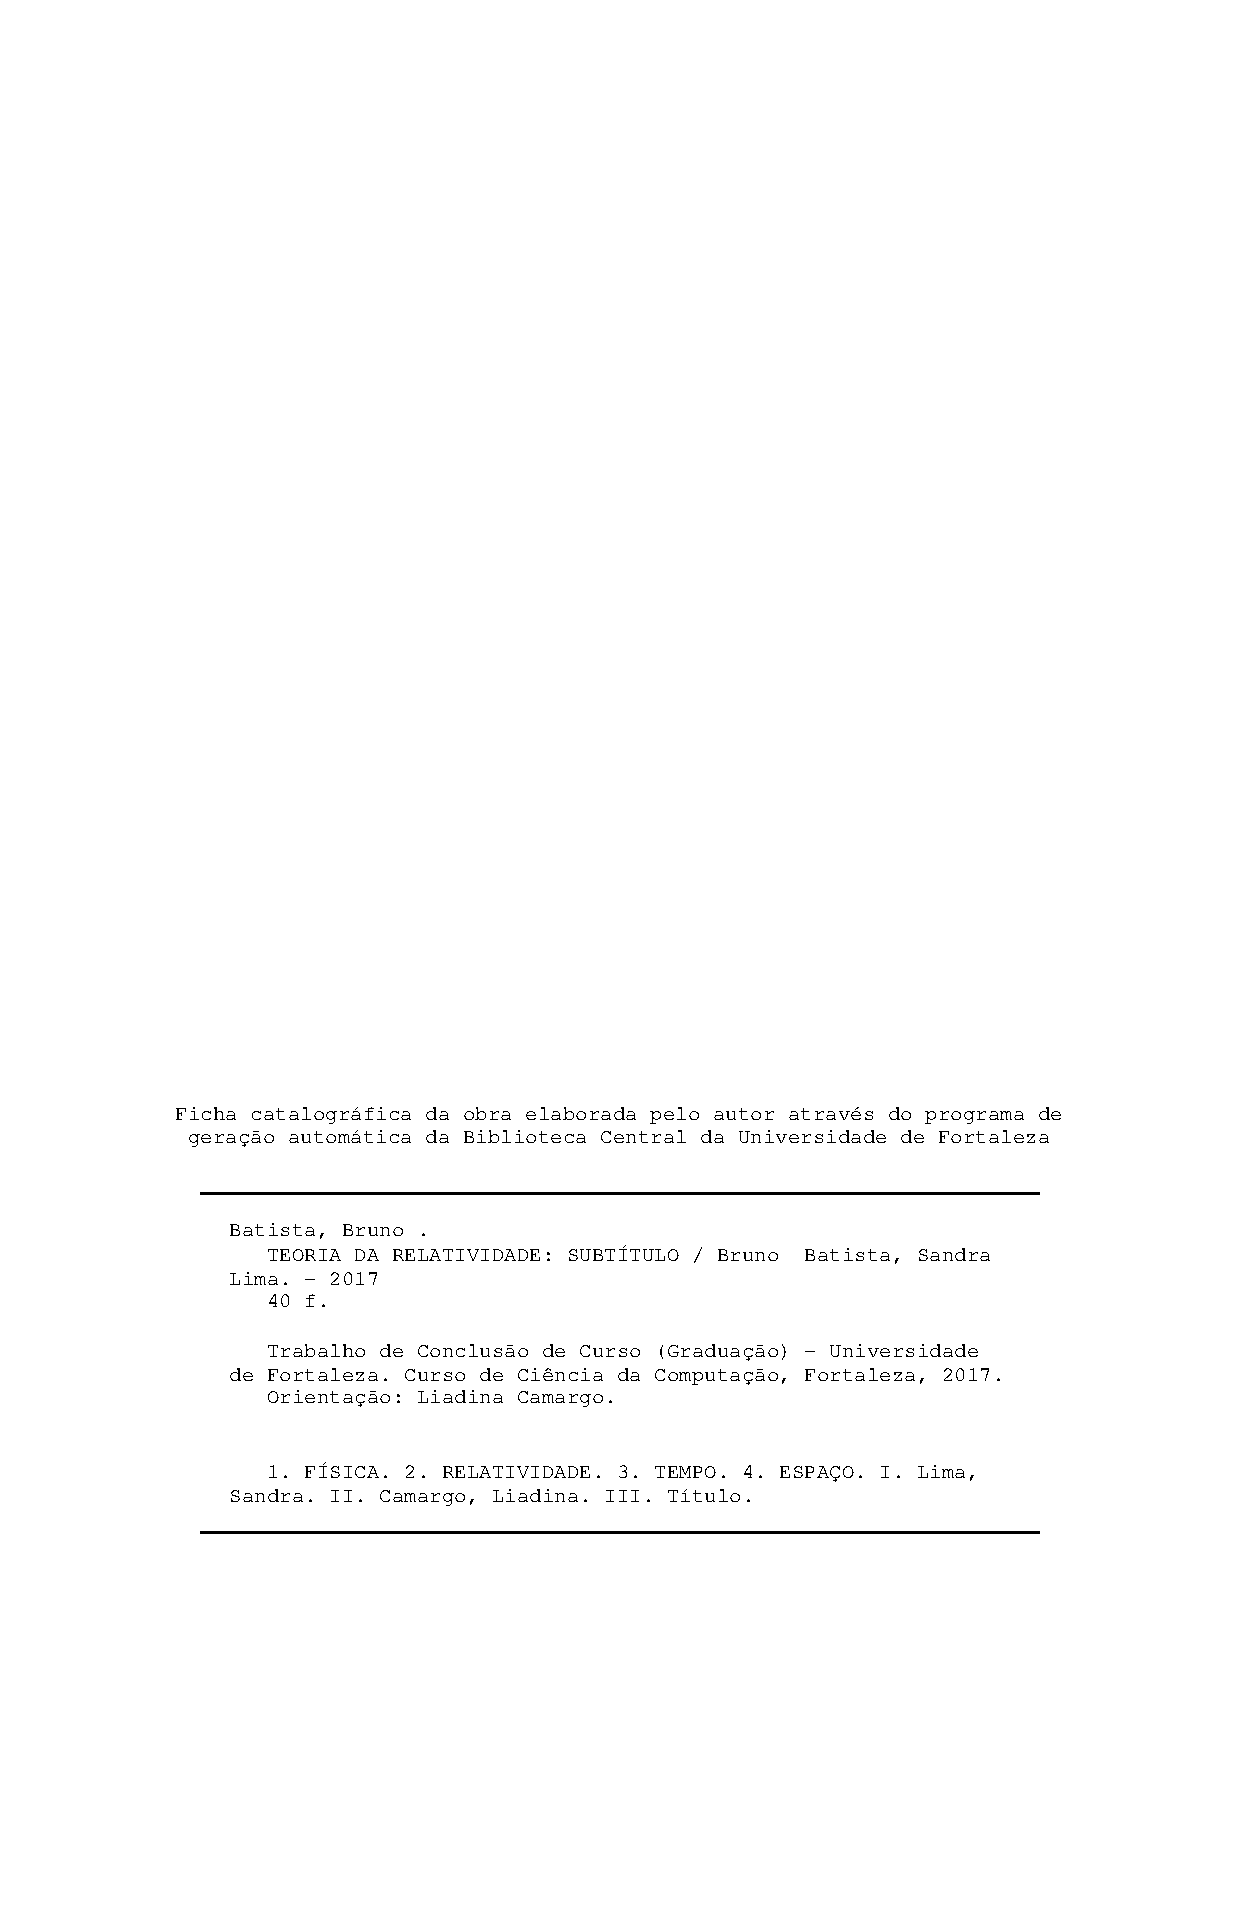
\includepdf{elementos-pre-textuais/folha-aprovacao.pdf}
		\imprimirfolhadeaprovacao

		\imprimirdedicatoria{elementos-pre-textuais/dedicatoria}
		\imprimiragradecimentos{elementos-pre-textuais/agradecimentos}
		\imprimirepigrafe{elementos-pre-textuais/epigrafe}
		\imprimirresumo{elementos-pre-textuais/resumo}
		\imprimirabstract{elementos-pre-textuais/abstract}
	\fi

	% Listas e sumário (comuns aos dois modos; cada lista sai vazia se o
	% documento não tiver o elemento correspondente).
	\imprimirlistadeilustracoes
	\imprimirlistadetabelas
	\imprimirlistadequadros
	\imprimirlistadealgoritmos
	\imprimirlistadecodigosfonte
	\imprimirlistadeabreviaturasesiglas
	\imprimirlistadesimbolos{elementos-pre-textuais/lista-de-simbolos}
	\imprimirsumario

	% Elementos textuais
	\textual
	\input{elementos-textuais/introducao}
	\input{elementos-textuais/revisao-de-literatura}
	\input{elementos-textuais/estado-da-arte}
	\input{elementos-textuais/material-e-metodos}
	\input{elementos-textuais/resultados-e-discussao}
	\input{elementos-textuais/consideracoes-finais}

	% Elementos pós-textuais
	% Todos abaixo aparecem no PDF SOMENTE quando há conteúdo correspondente;
	% caso contrário, são omitidos automaticamente (sem título em página vazia).

	% Referências: impressas se houver \cite/\citeonline no texto. Para forçar
	% a inclusão de uma obra não citada (ex.: a norma ABNT NBR 14724), adicione
	% \nocite{NBR14724:2005} antes da linha abaixo.
	\imprimirreferencias{elementos-pos-textuais/referencias}

	% Glossário: impresso se algum termo do glossário principal for usado no
	% texto com \gls/\Gls (siglas vão para a Lista de Abreviaturas e Siglas).
	\imprimirglossario

	% Apêndices: passe os \input dentro das chaves. Deixe vazio para omitir.
	\imprimirapendices{%
		\input{elementos-pos-textuais/apendices/exemplo-de-apendice}%
	}

	% Anexos: passe os \input dentro das chaves. Deixe vazio para omitir.
	\imprimiranexos{%
		\input{elementos-pos-textuais/anexos/exemplo-de-anexo}%
	}

	% Índice remissivo: impresso apenas se houver entradas \index{} no texto.
	\imprimirindice

\end{document}
 —
% veja ./gerar-exemplos.sh. Na compilação normal, valem os padrões abaixo.

\providecommand{\TipoDoc}{academico}
\tipodocumento{\TipoDoc}

% Subtipo: cada tipo tem seu próprio seletor. Edite o valor do SEU tipo abaixo
% (só o seletor correspondente ao \TipoDoc escolhido é aplicado):
\providecommand{\Nivel}{relatorio}      % academico:   tcc | monografia | dissertacao | tese | relatorio
\providecommand{\Serie}{relatorio}      % publicacao:  relatorio | boletim | comunicado | documento
\providecommand{\Categoria}{relatorio}  % corporativo: relatorio | analise
\ifacademico   \nivel{\Nivel}        \fi
\ifpublicacao  \serie{\Serie}        \fi
\ifcorporativo \categoria{\Categoria}\fi

% Caso não previsto? Defina os dois campos diretamente (é o que os seletores
% preenchem por baixo):
%   \subtitulodacapa{...}
%   \naturezadapublicacao{...}

% Remove as bordas vermelhas e verdes do PDF gerado
% Coloque 'sim' para remover

\removerbordasdohyperlink{sim}

% Adiciona a cor Azul a todos os hyperlinks

\cordohyperlink{nao}

%%%%%%%%%%%%%%%%%%%%%%%%%%%%%%%%%%%%%%%%%%%%%%%%%%%%%
%%       Informação sobre a Unidade Embrapa        %%
%%%%%%%%%%%%%%%%%%%%%%%%%%%%%%%%%%%%%%%%%%%%%%%%%%%%%

% Nome da unidade da Embrapa (ex.: Embrapa Agricultura Digital, Embrapa Cerrados, etc.)
\unidade{Embrapa Agricultura Digital}
\unidadesigla{CNPTIA}

% Área ou centro de pesquisa (opcional)
\centro{}

%%%%%%%%%%%%%%%%%%%%%%%%%%%%%%%%%%%%%%%%%%%%%%%%%%%%%
%%   Informação acadêmica (tipo 'academico')       %%
%%%%%%%%%%%%%%%%%%%%%%%%%%%%%%%%%%%%%%%%%%%%%%%%%%%%%

% Campos usados no modo academico. Os \providecommand permitem que os exemplos
% (exemplo-*.tex) os sobrescrevam via \def; na compilação normal, edite os
% valores aqui.

% Instituição de ensino (universidade/IES). Usada na capa e no preâmbulo.
\providecommand{\Instituicao}{Embrapa Agricultura Digital}
\instituicao{\Instituicao}

% Programa de pós-graduação ou curso (compõe o preâmbulo em tcc/monografia/
% dissertacao/tese; não usado no nível 'relatorio').
\providecommand{\ProgramaPesquisa}{}
\programapesquisa{\ProgramaPesquisa}

% Aparecem na folha de rosto apenas se preenchidas (qualquer nível academico):
\providecommand{\AreaPesquisa}{}   % Área de concentração
\areadepesquisa{\AreaPesquisa}
\providecommand{\LinhaPesquisa}{}  % Linha de pesquisa
\linhapesquisa{\LinhaPesquisa}

%%%%%%%%%%%%%%%%%%%%%%%%%%%%%%%%%%%%%%%%%%%%%%%%%%%%%
%%   Informação da série (tipo 'publicacao')       %%
%%%%%%%%%%%%%%%%%%%%%%%%%%%%%%%%%%%%%%%%%%%%%%%%%%%%%

% Número do documento na série (ex.: 123). Impresso na capa se preenchido.
\providecommand{\NumeroDocumento}{}
\numerodocumento{\NumeroDocumento}

%%%%%%%%%%%%%%%%%%%%%%%%%%%%%%%%%%%%%%%%%%%%%%%%%%%%%
%%     Informação relacionada ao documento         %%
%%%%%%%%%%%%%%%%%%%%%%%%%%%%%%%%%%%%%%%%%%%%%%%%%%%%%

% Preencha com os dados do seu trabalho
\autor{Maria Exemplo da Silva}
\titulo{Análise de um Problema de Pesquisa: Um Estudo de Caso Ilustrativo}
\data{2026}
\local{Campinas -- SP}

% Data de aprovação (se aplicável)
% Exemplo: \dataaprovacao{01 de janeiro de 2026}
\dataaprovacao{15 de junho de 2026}

%%%%%%%%%%%%%%%%%%%%%%%%%%%%%%%%%%%%%%%%%%%%%%%%%%%%%
%%     Informação sobre o Orientador/Supervisor    %%
%%%%%%%%%%%%%%%%%%%%%%%%%%%%%%%%%%%%%%%%%%%%%%%%%%%%%

% Preencha com os dados do orientador ou supervisor do trabalho
\orientador{João Orientador Exemplo}
\orientadories{Embrapa Agricultura Digital}
\orientadorcentro{}
\orientadorfeminino{nao} % Coloque 'sim' se for do sexo feminino

%%%%%%%%%%%%%%%%%%%%%%%%%%%%%%%%%%%%%%%%%%%%%%%%%%%%%
%%      Informação sobre o Co-orientador           %%
%%%%%%%%%%%%%%%%%%%%%%%%%%%%%%%%%%%%%%%%%%%%%%%%%%%%%

% Deixe o nome do coorientador em branco para remover do documento

\coorientador{}
\coorientadories{}
\coorientadorcentro{}
\coorientadorfeminino{nao} % Coloque 'sim' se for do sexo feminino

%%%%%%%%%%%%%%%%%%%%%%%%%%%%%%%%%%%%%%%%%%%%%%%%%%%%%
%%      Informação sobre a banca/revisores         %%
%%%%%%%%%%%%%%%%%%%%%%%%%%%%%%%%%%%%%%%%%%%%%%%%%%%%%

% Deixe o nome do membro em branco para remover da folha de aprovação
% Exemplo de uso:
% \membrodabancadois{Dr. Fulano de Tal}
% \membrodabancadoisies{Embrapa Cerrados}

\membrodabancadois{Ana Avaliadora Exemplo}
\membrodabancadoiscentro{}
\membrodabancadoisies{Universidade Federal de Exemplo}

\membrodabancatres{Carlos Revisor Exemplo}
\membrodabancatrescentro{}
\membrodabancatresies{Embrapa Agricultura Digital}

\membrodabancaquatro{}
\membrodabancaquatrocentro{}
\membrodabancaquatroies{}

\membrodabancacinco{}
\membrodabancacincocentro{}
\membrodabancacincoies{}

\membrodabancaseis{}
\membrodabancaseiscentro{}
\membrodabancaseisies{}

%%%%%%%%%%%%%%%%%%%%%%%%%%%%%%%%%%%%%%%%%%%%%%%%%%%%%
%%        Informação da Ficha Catalográfica        %%
%%%%%%%%%%%%%%%%%%%%%%%%%%%%%%%%%%%%%%%%%%%%%%%%%%%%%

% A ficha catalográfica é gerada automaticamente em LaTeX a partir dos campos
% abaixo — não é mais necessário anexar um PDF externo. Os dados de
% classificação (CDD/CDU), os descritores de assunto e o registro CRB do
% bibliotecário devem ser fornecidos por um(a) bibliotecário(a).

% Nome do autor invertido para a entrada principal (Sobrenome, Nome).
% Se ficar em branco, será usado o \autor definido acima.
\autorinvertido{Silva, Maria Exemplo da}

% Dados da publicação
\edicao{1. ed.}           % Ex.: 1. ed. (deixe em branco se não houver)
\editora{Embrapa}         % Editora responsável
\numeropaginas{30}        % Número total de páginas (ex.: 85)
\ilustracao{il. color.}   % Ex.: il. / il. color. (deixe em branco se não houver)
\dimensao{21 cm}          % Altura da publicação

% Informações complementares
\isbn{978-65-00000-00-0}  % ISBN, se houver
\notaficha{Documento de exemplo gerado com o template EmbrapaTex.} % Nota livre (ex.: tipo do trabalho, orientador)
\incluibibliografia{sim}  % 'sim' imprime "Inclui bibliografia."

% Dados fornecidos pelo(a) bibliotecário(a)
\descritores{1. Pesquisa. 2. Metodologia científica. 3. Documentação técnica. I. Título.} % Ex.: 1. Agricultura digital. 2. Sensoriamento remoto. I. Título.
\cdd{001.42}              % Classificação Decimal de Dewey (ex.: 630)
\cdu{}                    % Classificação Decimal Universal (opcional)
\bibliotecario{Bibliotecário(a) Exemplo} % Nome do(a) bibliotecário(a)
\crb{CRB-8/0000}          % Registro profissional (ex.: CRB-1/1234)

\begin{document}

	% Elementos pré-textuais
	\imprimircapa
	\imprimirfolhaderosto

	%%%%%%%%%%%%%%%%%%%%%%%%%%%%%%%%%%%%%%%%%%%%%%%%%%%%%%%%%%%%%%%%%%%%%%%%%%
	%%  Os elementos pré-textuais variam conforme \tipodocumento:           %%
	%%   - corporativo  -> sumário executivo (modo empresarial)             %%
	%%   - demais tipos -> estrutura acadêmica/ABNT completa                %%
	%%  O condicional \ifcorporativo é definido em lib/embrapatex.sty.      %%
	%%%%%%%%%%%%%%%%%%%%%%%%%%%%%%%%%%%%%%%%%%%%%%%%%%%%%%%%%%%%%%%%%%%%%%%%%%
	\ifcorporativo
		%% ----- Modo corporativo/empresarial -----
		\imprimirsumarioexecutivo{elementos-pre-textuais/sumario-executivo}
	\else
		%% ----- Modo acadêmico/científico (ABNT) -----
		\imprimirfichacatalografica
		\imprimirerrata{elementos-pre-textuais/errata}

		%%%%%%%%%%%%%%%%%%%%%%%%%%%%%%%%%%%%%%%%%%%%%%%%%%%%%%%%%%%%%%%%%%%%%%
		%%  Folha de aprovação:                                             %%
		%%  Caso possua uma folha de aprovação assinada em PDF,             %%
		%%  descomente a linha \includepdf abaixo e comente                 %%
		%%  a linha \imprimirfolhadeaprovacao.                              %%
		%%%%%%%%%%%%%%%%%%%%%%%%%%%%%%%%%%%%%%%%%%%%%%%%%%%%%%%%%%%%%%%%%%%%%%

		%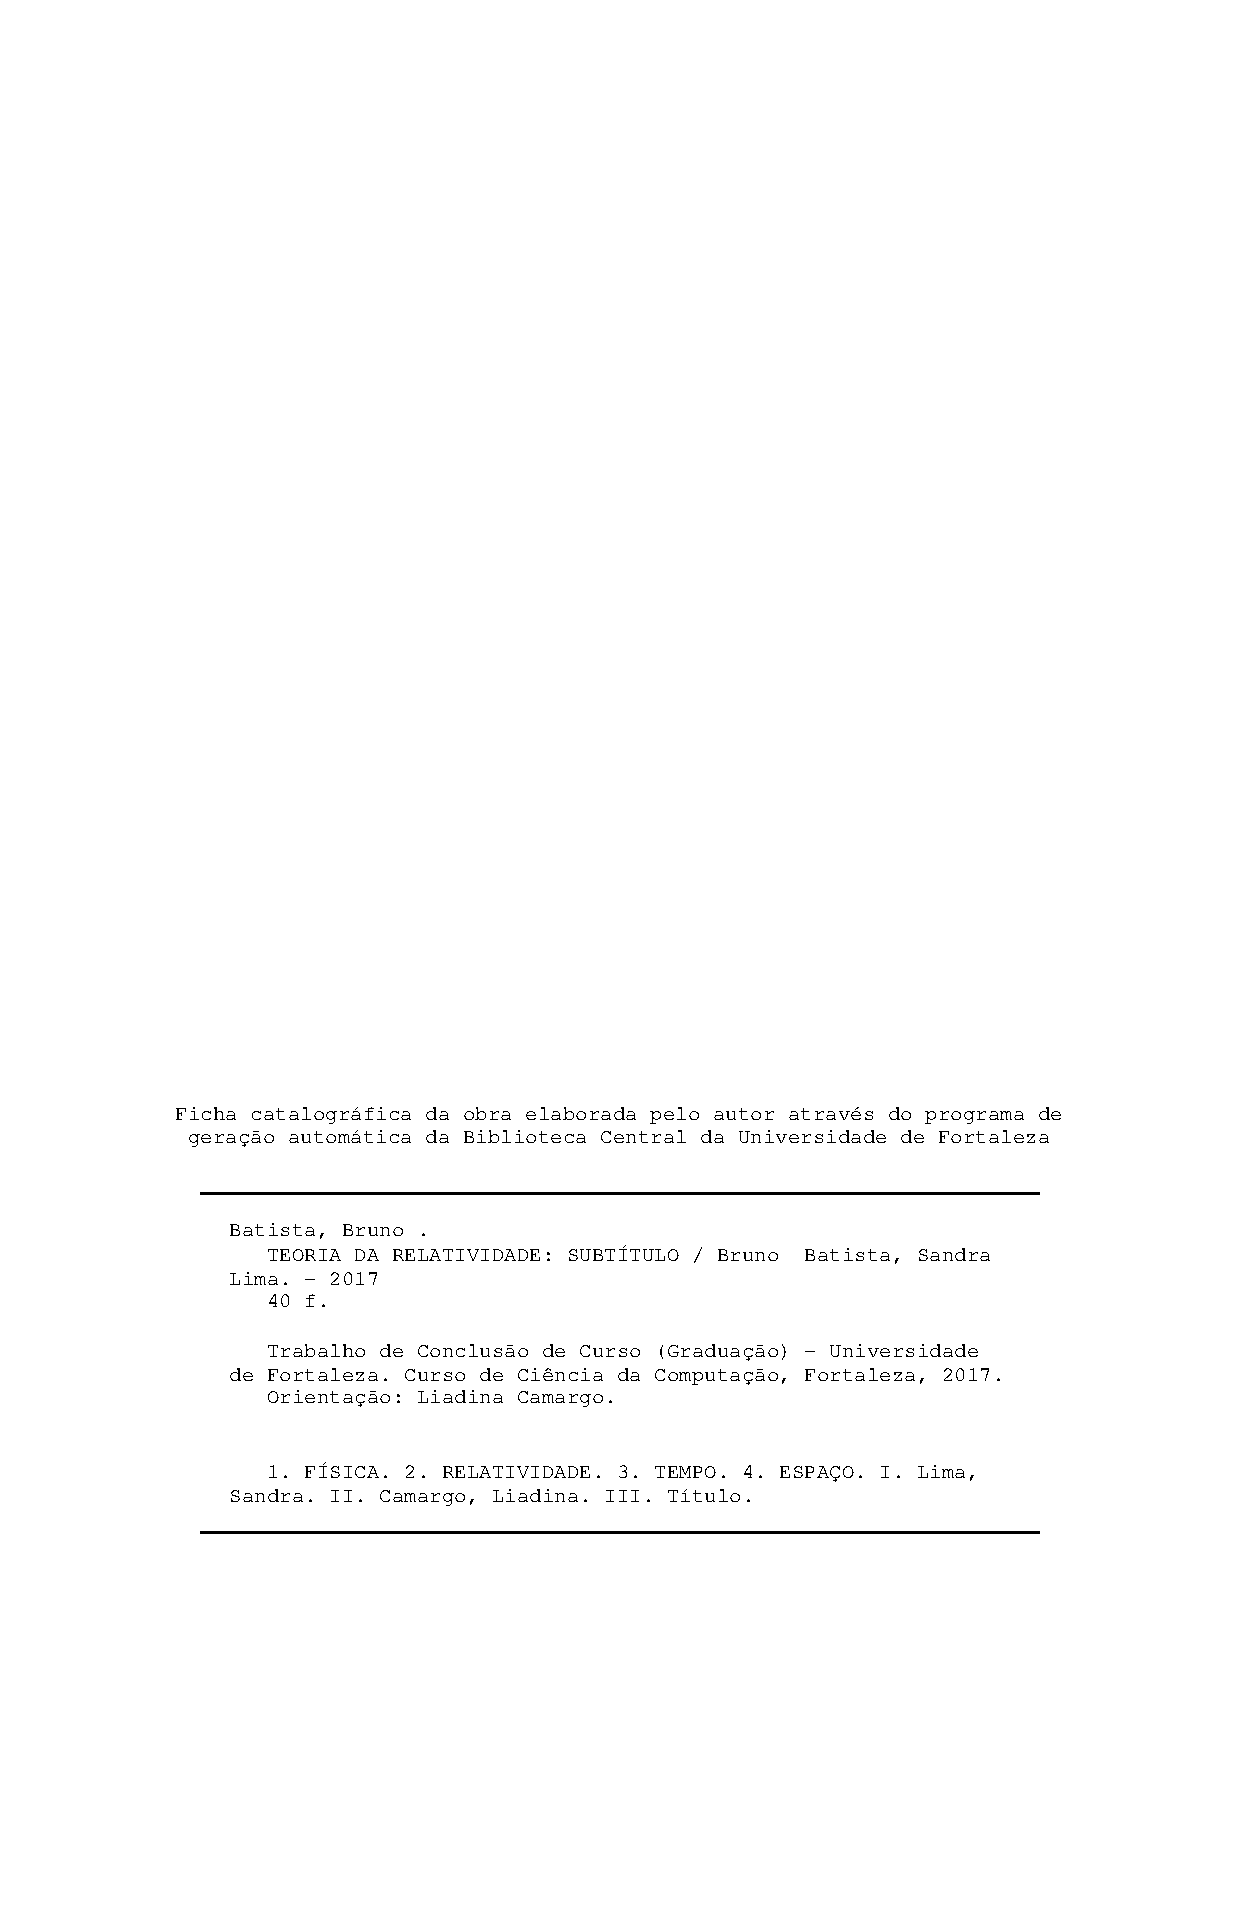
\includepdf{elementos-pre-textuais/folha-aprovacao.pdf}
		\imprimirfolhadeaprovacao

		\imprimirdedicatoria{elementos-pre-textuais/dedicatoria}
		\imprimiragradecimentos{elementos-pre-textuais/agradecimentos}
		\imprimirepigrafe{elementos-pre-textuais/epigrafe}
		\imprimirresumo{elementos-pre-textuais/resumo}
		\imprimirabstract{elementos-pre-textuais/abstract}
	\fi

	% Listas e sumário (comuns aos dois modos; cada lista sai vazia se o
	% documento não tiver o elemento correspondente).
	\imprimirlistadeilustracoes
	\imprimirlistadetabelas
	\imprimirlistadequadros
	\imprimirlistadealgoritmos
	\imprimirlistadecodigosfonte
	\imprimirlistadeabreviaturasesiglas
	\imprimirlistadesimbolos{elementos-pre-textuais/lista-de-simbolos}
	\imprimirsumario

	% Elementos textuais
	\textual
	\chapter{Introdução}
\label{cap:introducao}

% Descreva aqui o contexto geral do trabalho, apresentando o tema,
% a problemática e a justificativa da pesquisa.

% [Insira o texto da introdução aqui]

\section{Justificativa}
\label{sec:justificativa}

% Apresente a relevância e a motivação para a realização deste trabalho.

% [Insira a justificativa aqui]

\section{Objetivos}
\label{sec:objetivos}

% Apresente os objetivos geral e específicos do trabalho.

\subsection{Objetivo Geral}
\label{sec:objetivo-geral}

% [Insira o objetivo geral aqui]

\subsection{Objetivos Específicos}
\label{sec:objetivos-especificos}

% Liste os objetivos específicos usando alíneas:
%
% \begin{alineas}
% 	\item Objetivo específico 1;
% 	\item Objetivo específico 2;
% 	\item Objetivo específico 3.
% \end{alineas}

% [Insira os objetivos específicos aqui]
	\chapter{Revisão de Literatura}
\label{cap:revisao-de-literatura}

% Apresente aqui a fundamentação teórica do trabalho.
% Realize uma revisão bibliográfica dos principais conceitos,
% teorias e trabalhos anteriores relacionados ao tema.

% [Insira o texto da revisão de literatura aqui]

\section{Tema A}
\label{sec:tema-a}

% [Insira o conteúdo da primeira seção aqui]

% Dica: Para inserir uma figura, use o seguinte modelo:
%
% \begin{figure}[!htbp]
%     \centering
%     \EMBRAPAfig{
%         \Caption{\label{fig:exemplo} Legenda da figura}
%     }{
%         \includegraphics[width=8cm]{figuras/nome-da-figura}
%     }{
%         \Fonte{Elaborado pelo autor}
%     }
% \end{figure}

\section{Tema B}
\label{sec:tema-b}

% [Insira o conteúdo da segunda seção aqui]

% Dica: Para inserir uma tabela, use o seguinte modelo:
%
% \begin{table}[!htbp]
%     \centering
%     \Caption{\label{tab:exemplo} Legenda da tabela}
%     \EMBRAPAtab{}{
%         \begin{tabular}{cll}
%             \toprule
%             Coluna 1 & Coluna 2 & Coluna 3 \\
%             \midrule \midrule
%             Dado 1 & Dado 2 & Dado 3 \\
%             \bottomrule
%         \end{tabular}
%     }{
%         \Fonte{Elaborado pelo autor}
%     }
% \end{table}

	\chapter{Estado da Arte}
\label{cap:estado-da-arte}

% Apresente aqui uma revisão dos trabalhos e pesquisas mais recentes
% relacionados ao tema, destacando as contribuições e lacunas existentes.

% [Insira o texto do estado da arte aqui]

\section{Trabalho/Pesquisa A}
\label{sec:trabalho-a}

% [Descreva o primeiro trabalho relacionado]

\section{Trabalho/Pesquisa B}
\label{sec:trabalho-b}

% [Descreva o segundo trabalho relacionado]

% Dica: Para inserir um quadro comparativo, use o seguinte modelo:
%
% \begin{quadro}[!htbp]
%     \centering
%     \Caption{\label{qua:comparativo} Legenda do quadro}
%     \EMBRAPAqua{}{
%         \begin{tabular}{|c|c|c|}
%             \hline
%             Critério & Trabalho A & Trabalho B \\
%             \hline
%             Critério 1 & Valor & Valor \\
%             \hline
%         \end{tabular}
%     }{
%         \Fonte{Elaborado pelo autor}
%     }
% \end{quadro}

	\chapter{Material e Métodos}
\label{cap:material-e-metodos}

% Descreva aqui os materiais utilizados e os métodos empregados
% na realização da pesquisa. Inclua informações sobre:
% - Área de estudo / local do experimento
% - Materiais e equipamentos
% - Delineamento experimental
% - Procedimentos analíticos
% - Análises estatísticas

% [Insira o texto de material e métodos aqui]

\section{Área de Estudo}
\label{sec:area-de-estudo}

% [Descreva a área ou local onde o trabalho foi realizado]

\section{Procedimentos Metodológicos}
\label{sec:procedimentos-metodologicos}

% [Descreva os procedimentos utilizados]

% Dica: Para inserir um algoritmo, use o seguinte modelo:
%
% \begin{algorithm}[h!]
%     \SetSpacedAlgorithm
%     \caption{\label{alg:exemplo}Descrição do Algoritmo}
%     \Entrada{Entrada do Algoritmo}
%     \Saida{Saída do Algoritmo}
%     \Inicio{
%         Passo 1\;
%         Passo 2\;
%     }
% \end{algorithm}

\section{Análise dos Dados}
\label{sec:analise-dos-dados}

% [Descreva como os dados foram analisados]

% Dica: Para inserir fórmulas matemáticas:
%
% \begin{equation}
%     \begin{aligned}
%         y = ax + b
%     \end{aligned}
% \end{equation}

	\chapter{Resultados e Discussão}
\label{cap:resultados-e-discussao}

% Apresente aqui os resultados obtidos na pesquisa e discuta-os
% à luz da literatura revisada. Inclua figuras, tabelas e gráficos
% conforme necessário.

% [Insira os resultados e a discussão aqui]

\section{Resultados}
\label{sec:resultados}

% [Apresente os resultados obtidos]

\section{Discussão}
\label{sec:discussao}

% [Discuta os resultados à luz da literatura]

	\chapter{Considerações Finais}
\label{cap:consideracoes-finais}

% Apresente aqui as conclusões do trabalho, retomando os objetivos
% propostos e avaliando se foram alcançados.

% [Insira as considerações finais aqui]

\section{Contribuições do Trabalho}
\label{sec:contribuicoes-do-trabalho}

% [Descreva as principais contribuições]

\section{Limitações}
\label{sec:limitacoes}

% [Descreva as limitações encontradas]

\section{Recomendações e Trabalhos Futuros}
\label{sec:recomendacoes-e-trabalhos-futuros}

% [Apresente recomendações e sugestões para trabalhos futuros]


	% Elementos pós-textuais
	% Todos abaixo aparecem no PDF SOMENTE quando há conteúdo correspondente;
	% caso contrário, são omitidos automaticamente (sem título em página vazia).

	% Referências: impressas se houver \cite/\citeonline no texto. Para forçar
	% a inclusão de uma obra não citada (ex.: a norma ABNT NBR 14724), adicione
	% \nocite{NBR14724:2005} antes da linha abaixo.
	\imprimirreferencias{elementos-pos-textuais/referencias}

	% Glossário: impresso se algum termo do glossário principal for usado no
	% texto com \gls/\Gls (siglas vão para a Lista de Abreviaturas e Siglas).
	\imprimirglossario

	% Apêndices: passe os \input dentro das chaves. Deixe vazio para omitir.
	\imprimirapendices{%
		\apendice{Exemplo de Apêndice}
\label{ap:exemplo-de-apendice}

% Apêndice é um texto ou documento elaborado pelo autor.
% Adicione aqui o conteúdo do apêndice.

% [Insira o conteúdo do apêndice aqui]
Este apêndice apresenta material complementar elaborado pelo autor, como dados adicionais, formulários ou detalhamentos que apoiam o texto principal sem comprometer a sua fluidez.
%
	}

	% Anexos: passe os \input dentro das chaves. Deixe vazio para omitir.
	\imprimiranexos{%
		\anexo{Exemplo de Anexo}
\label{an:exemplo-de-anexo}

% Anexo é um texto ou documento não elaborado pelo autor.
% Adicione aqui o conteúdo do anexo.

% [Insira o conteúdo do anexo aqui]%
	}

	% Índice remissivo: impresso apenas se houver entradas \index{} no texto.
	\imprimirindice

\end{document}
 —
% veja ./gerar-exemplos.sh. Na compilação normal, valem os padrões abaixo.

\providecommand{\TipoDoc}{academico}
\tipodocumento{\TipoDoc}

% Subtipo: cada tipo tem seu próprio seletor. Edite o valor do SEU tipo abaixo
% (só o seletor correspondente ao \TipoDoc escolhido é aplicado):
\providecommand{\Nivel}{relatorio}      % academico:   tcc | monografia | dissertacao | tese | relatorio
\providecommand{\Serie}{relatorio}      % publicacao:  relatorio | boletim | comunicado | documento
\providecommand{\Categoria}{relatorio}  % corporativo: relatorio | analise
\ifacademico   \nivel{\Nivel}        \fi
\ifpublicacao  \serie{\Serie}        \fi
\ifcorporativo \categoria{\Categoria}\fi

% Caso não previsto? Defina os dois campos diretamente (é o que os seletores
% preenchem por baixo):
%   \subtitulodacapa{...}
%   \naturezadapublicacao{...}

% Remove as bordas vermelhas e verdes do PDF gerado
% Coloque 'sim' para remover

\removerbordasdohyperlink{sim}

% Adiciona a cor Azul a todos os hyperlinks

\cordohyperlink{nao}

%%%%%%%%%%%%%%%%%%%%%%%%%%%%%%%%%%%%%%%%%%%%%%%%%%%%%
%%       Informação sobre a Unidade Embrapa        %%
%%%%%%%%%%%%%%%%%%%%%%%%%%%%%%%%%%%%%%%%%%%%%%%%%%%%%

% Nome da unidade da Embrapa (ex.: Embrapa Agricultura Digital, Embrapa Cerrados, etc.)
\unidade{Embrapa Agricultura Digital}
\unidadesigla{CNPTIA}

% Área ou centro de pesquisa (opcional)
\centro{}

%%%%%%%%%%%%%%%%%%%%%%%%%%%%%%%%%%%%%%%%%%%%%%%%%%%%%
%%   Informação acadêmica (tipo 'academico')       %%
%%%%%%%%%%%%%%%%%%%%%%%%%%%%%%%%%%%%%%%%%%%%%%%%%%%%%

% Campos usados no modo academico. Os \providecommand permitem que os exemplos
% (exemplo-*.tex) os sobrescrevam via \def; na compilação normal, edite os
% valores aqui.

% Instituição de ensino (universidade/IES). Usada na capa e no preâmbulo.
\providecommand{\Instituicao}{Embrapa Agricultura Digital}
\instituicao{\Instituicao}

% Programa de pós-graduação ou curso (compõe o preâmbulo em tcc/monografia/
% dissertacao/tese; não usado no nível 'relatorio').
\providecommand{\ProgramaPesquisa}{}
\programapesquisa{\ProgramaPesquisa}

% Aparecem na folha de rosto apenas se preenchidas (qualquer nível academico):
\providecommand{\AreaPesquisa}{}   % Área de concentração
\areadepesquisa{\AreaPesquisa}
\providecommand{\LinhaPesquisa}{}  % Linha de pesquisa
\linhapesquisa{\LinhaPesquisa}

%%%%%%%%%%%%%%%%%%%%%%%%%%%%%%%%%%%%%%%%%%%%%%%%%%%%%
%%   Informação da série (tipo 'publicacao')       %%
%%%%%%%%%%%%%%%%%%%%%%%%%%%%%%%%%%%%%%%%%%%%%%%%%%%%%

% Número do documento na série (ex.: 123). Impresso na capa se preenchido.
\providecommand{\NumeroDocumento}{}
\numerodocumento{\NumeroDocumento}

%%%%%%%%%%%%%%%%%%%%%%%%%%%%%%%%%%%%%%%%%%%%%%%%%%%%%
%%     Informação relacionada ao documento         %%
%%%%%%%%%%%%%%%%%%%%%%%%%%%%%%%%%%%%%%%%%%%%%%%%%%%%%

% Preencha com os dados do seu trabalho
\autor{Maria Exemplo da Silva}
\titulo{Análise de um Problema de Pesquisa: Um Estudo de Caso Ilustrativo}
\data{2026}
\local{Campinas -- SP}

% Data de aprovação (se aplicável)
% Exemplo: \dataaprovacao{01 de janeiro de 2026}
\dataaprovacao{15 de junho de 2026}

%%%%%%%%%%%%%%%%%%%%%%%%%%%%%%%%%%%%%%%%%%%%%%%%%%%%%
%%     Informação sobre o Orientador/Supervisor    %%
%%%%%%%%%%%%%%%%%%%%%%%%%%%%%%%%%%%%%%%%%%%%%%%%%%%%%

% Preencha com os dados do orientador ou supervisor do trabalho
\orientador{João Orientador Exemplo}
\orientadories{Embrapa Agricultura Digital}
\orientadorcentro{}
\orientadorfeminino{nao} % Coloque 'sim' se for do sexo feminino

%%%%%%%%%%%%%%%%%%%%%%%%%%%%%%%%%%%%%%%%%%%%%%%%%%%%%
%%      Informação sobre o Co-orientador           %%
%%%%%%%%%%%%%%%%%%%%%%%%%%%%%%%%%%%%%%%%%%%%%%%%%%%%%

% Deixe o nome do coorientador em branco para remover do documento

\coorientador{}
\coorientadories{}
\coorientadorcentro{}
\coorientadorfeminino{nao} % Coloque 'sim' se for do sexo feminino

%%%%%%%%%%%%%%%%%%%%%%%%%%%%%%%%%%%%%%%%%%%%%%%%%%%%%
%%      Informação sobre a banca/revisores         %%
%%%%%%%%%%%%%%%%%%%%%%%%%%%%%%%%%%%%%%%%%%%%%%%%%%%%%

% Deixe o nome do membro em branco para remover da folha de aprovação
% Exemplo de uso:
% \membrodabancadois{Dr. Fulano de Tal}
% \membrodabancadoisies{Embrapa Cerrados}

\membrodabancadois{Ana Avaliadora Exemplo}
\membrodabancadoiscentro{}
\membrodabancadoisies{Universidade Federal de Exemplo}

\membrodabancatres{Carlos Revisor Exemplo}
\membrodabancatrescentro{}
\membrodabancatresies{Embrapa Agricultura Digital}

\membrodabancaquatro{}
\membrodabancaquatrocentro{}
\membrodabancaquatroies{}

\membrodabancacinco{}
\membrodabancacincocentro{}
\membrodabancacincoies{}

\membrodabancaseis{}
\membrodabancaseiscentro{}
\membrodabancaseisies{}

%%%%%%%%%%%%%%%%%%%%%%%%%%%%%%%%%%%%%%%%%%%%%%%%%%%%%
%%        Informação da Ficha Catalográfica        %%
%%%%%%%%%%%%%%%%%%%%%%%%%%%%%%%%%%%%%%%%%%%%%%%%%%%%%

% A ficha catalográfica é gerada automaticamente em LaTeX a partir dos campos
% abaixo — não é mais necessário anexar um PDF externo. Os dados de
% classificação (CDD/CDU), os descritores de assunto e o registro CRB do
% bibliotecário devem ser fornecidos por um(a) bibliotecário(a).

% Nome do autor invertido para a entrada principal (Sobrenome, Nome).
% Se ficar em branco, será usado o \autor definido acima.
\autorinvertido{Silva, Maria Exemplo da}

% Dados da publicação
\edicao{1. ed.}           % Ex.: 1. ed. (deixe em branco se não houver)
\editora{Embrapa}         % Editora responsável
\numeropaginas{30}        % Número total de páginas (ex.: 85)
\ilustracao{il. color.}   % Ex.: il. / il. color. (deixe em branco se não houver)
\dimensao{21 cm}          % Altura da publicação

% Informações complementares
\isbn{978-65-00000-00-0}  % ISBN, se houver
\notaficha{Documento de exemplo gerado com o template EmbrapaTex.} % Nota livre (ex.: tipo do trabalho, orientador)
\incluibibliografia{sim}  % 'sim' imprime "Inclui bibliografia."

% Dados fornecidos pelo(a) bibliotecário(a)
\descritores{1. Pesquisa. 2. Metodologia científica. 3. Documentação técnica. I. Título.} % Ex.: 1. Agricultura digital. 2. Sensoriamento remoto. I. Título.
\cdd{001.42}              % Classificação Decimal de Dewey (ex.: 630)
\cdu{}                    % Classificação Decimal Universal (opcional)
\bibliotecario{Bibliotecário(a) Exemplo} % Nome do(a) bibliotecário(a)
\crb{CRB-8/0000}          % Registro profissional (ex.: CRB-1/1234)

\begin{document}

	% Elementos pré-textuais
	\imprimircapa
	\imprimirfolhaderosto

	%%%%%%%%%%%%%%%%%%%%%%%%%%%%%%%%%%%%%%%%%%%%%%%%%%%%%%%%%%%%%%%%%%%%%%%%%%
	%%  Os elementos pré-textuais variam conforme \tipodocumento:           %%
	%%   - corporativo  -> sumário executivo (modo empresarial)             %%
	%%   - demais tipos -> estrutura acadêmica/ABNT completa                %%
	%%  O condicional \ifcorporativo é definido em lib/embrapatex.sty.      %%
	%%%%%%%%%%%%%%%%%%%%%%%%%%%%%%%%%%%%%%%%%%%%%%%%%%%%%%%%%%%%%%%%%%%%%%%%%%
	\ifcorporativo
		%% ----- Modo corporativo/empresarial -----
		\imprimirsumarioexecutivo{elementos-pre-textuais/sumario-executivo}
	\else
		%% ----- Modo acadêmico/científico (ABNT) -----
		\imprimirfichacatalografica
		\imprimirerrata{elementos-pre-textuais/errata}

		%%%%%%%%%%%%%%%%%%%%%%%%%%%%%%%%%%%%%%%%%%%%%%%%%%%%%%%%%%%%%%%%%%%%%%
		%%  Folha de aprovação:                                             %%
		%%  Caso possua uma folha de aprovação assinada em PDF,             %%
		%%  descomente a linha \includepdf abaixo e comente                 %%
		%%  a linha \imprimirfolhadeaprovacao.                              %%
		%%%%%%%%%%%%%%%%%%%%%%%%%%%%%%%%%%%%%%%%%%%%%%%%%%%%%%%%%%%%%%%%%%%%%%

		%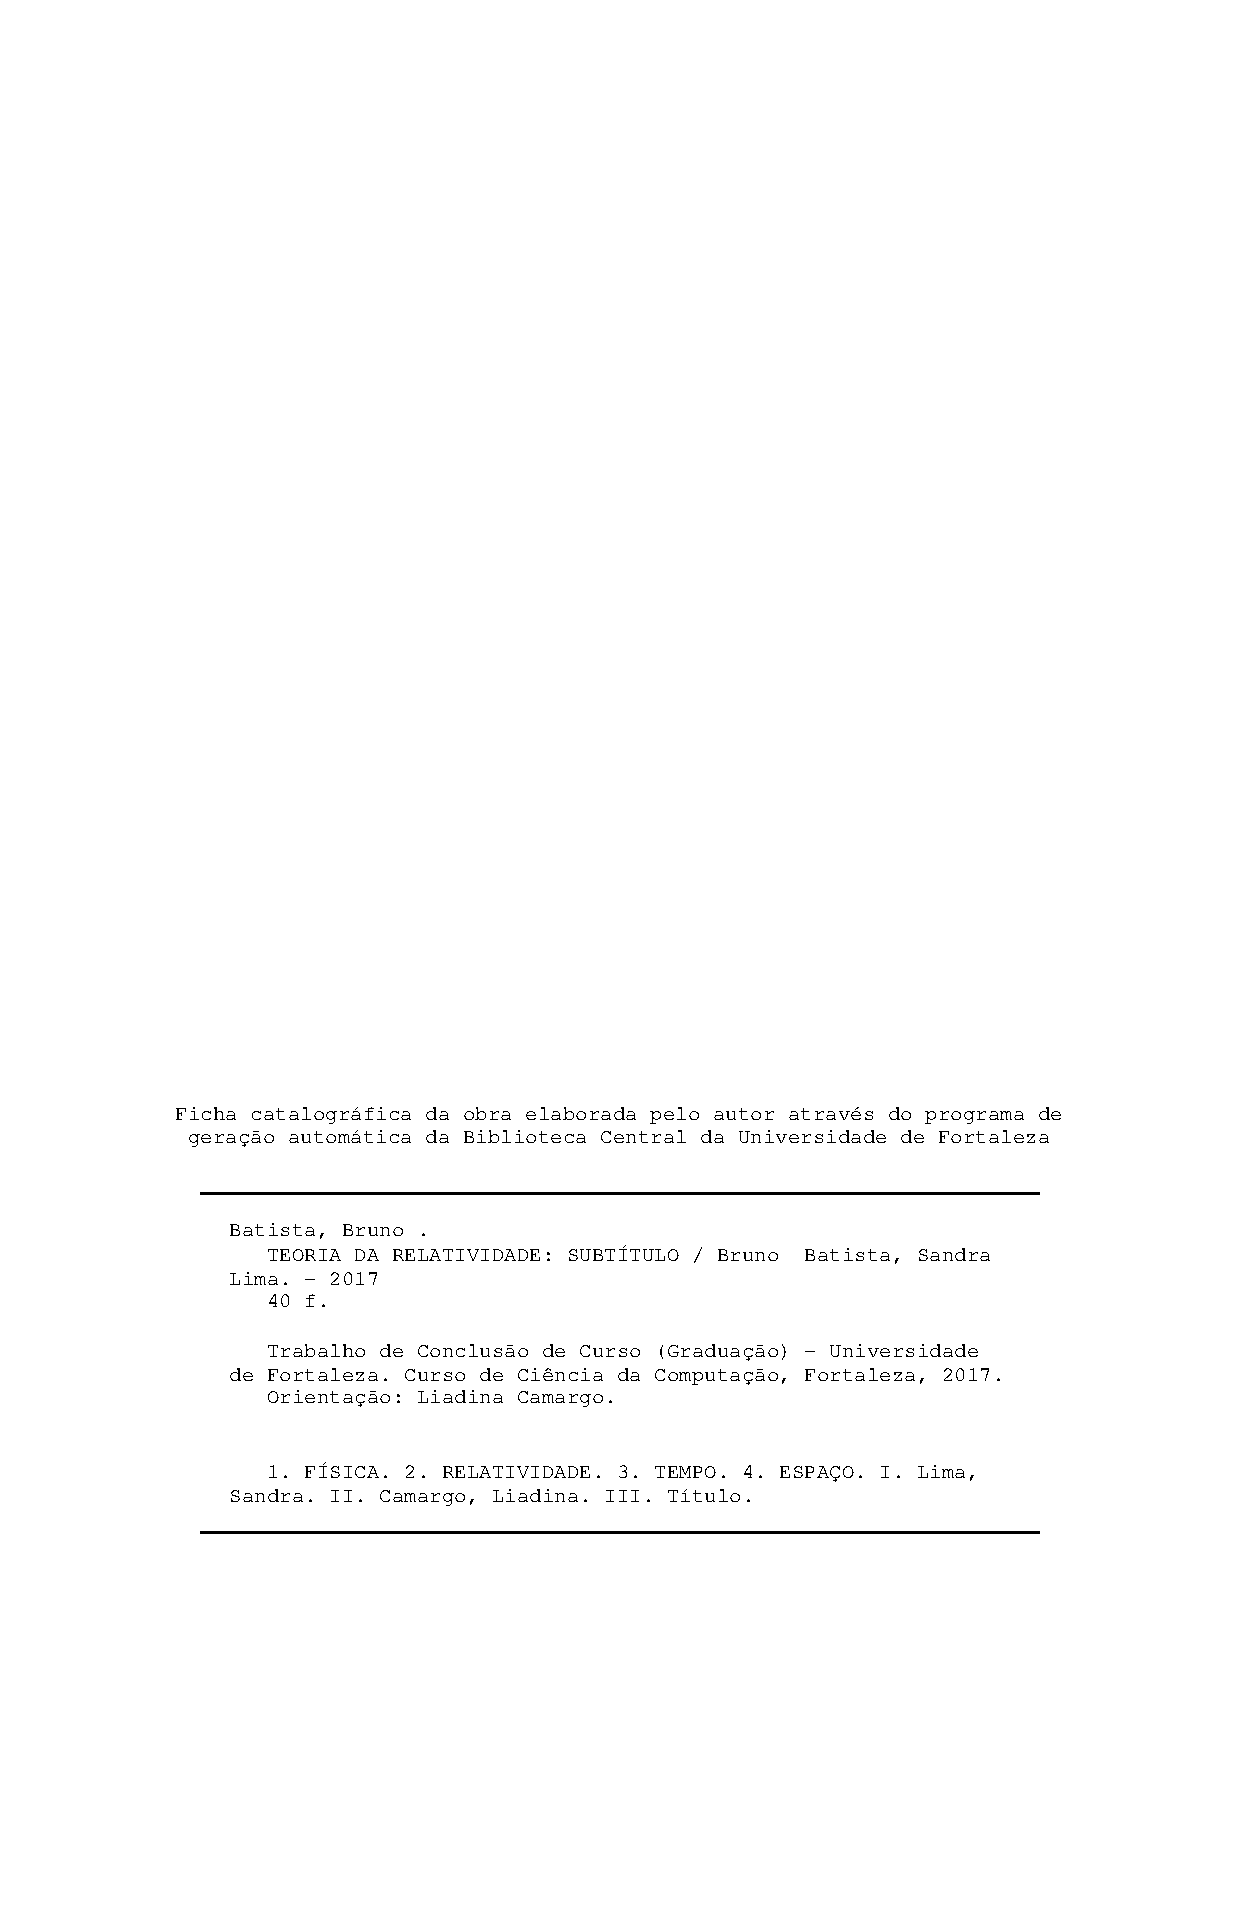
\includepdf{elementos-pre-textuais/folha-aprovacao.pdf}
		\imprimirfolhadeaprovacao

		\imprimirdedicatoria{elementos-pre-textuais/dedicatoria}
		\imprimiragradecimentos{elementos-pre-textuais/agradecimentos}
		\imprimirepigrafe{elementos-pre-textuais/epigrafe}
		\imprimirresumo{elementos-pre-textuais/resumo}
		\imprimirabstract{elementos-pre-textuais/abstract}
	\fi

	% Listas e sumário (comuns aos dois modos; cada lista sai vazia se o
	% documento não tiver o elemento correspondente).
	\imprimirlistadeilustracoes
	\imprimirlistadetabelas
	\imprimirlistadequadros
	\imprimirlistadealgoritmos
	\imprimirlistadecodigosfonte
	\imprimirlistadeabreviaturasesiglas
	\imprimirlistadesimbolos{elementos-pre-textuais/lista-de-simbolos}
	\imprimirsumario

	% Elementos textuais
	\textual
	\chapter{Introdução}
\label{cap:introducao}

% Descreva aqui o contexto geral do trabalho, apresentando o tema,
% a problemática e a justificativa da pesquisa.

% [Insira o texto da introdução aqui]

\section{Justificativa}
\label{sec:justificativa}

% Apresente a relevância e a motivação para a realização deste trabalho.

% [Insira a justificativa aqui]

\section{Objetivos}
\label{sec:objetivos}

% Apresente os objetivos geral e específicos do trabalho.

\subsection{Objetivo Geral}
\label{sec:objetivo-geral}

% [Insira o objetivo geral aqui]

\subsection{Objetivos Específicos}
\label{sec:objetivos-especificos}

% Liste os objetivos específicos usando alíneas:
%
% \begin{alineas}
% 	\item Objetivo específico 1;
% 	\item Objetivo específico 2;
% 	\item Objetivo específico 3.
% \end{alineas}

% [Insira os objetivos específicos aqui]
	\chapter{Revisão de Literatura}
\label{cap:revisao-de-literatura}

% Apresente aqui a fundamentação teórica do trabalho.
% Realize uma revisão bibliográfica dos principais conceitos,
% teorias e trabalhos anteriores relacionados ao tema.

% [Insira o texto da revisão de literatura aqui]

\section{Tema A}
\label{sec:tema-a}

% [Insira o conteúdo da primeira seção aqui]

% Dica: Para inserir uma figura, use o seguinte modelo:
%
% \begin{figure}[!htbp]
%     \centering
%     \EMBRAPAfig{
%         \Caption{\label{fig:exemplo} Legenda da figura}
%     }{
%         \includegraphics[width=8cm]{figuras/nome-da-figura}
%     }{
%         \Fonte{Elaborado pelo autor}
%     }
% \end{figure}

\section{Tema B}
\label{sec:tema-b}

% [Insira o conteúdo da segunda seção aqui]

% Dica: Para inserir uma tabela, use o seguinte modelo:
%
% \begin{table}[!htbp]
%     \centering
%     \Caption{\label{tab:exemplo} Legenda da tabela}
%     \EMBRAPAtab{}{
%         \begin{tabular}{cll}
%             \toprule
%             Coluna 1 & Coluna 2 & Coluna 3 \\
%             \midrule \midrule
%             Dado 1 & Dado 2 & Dado 3 \\
%             \bottomrule
%         \end{tabular}
%     }{
%         \Fonte{Elaborado pelo autor}
%     }
% \end{table}

	\chapter{Estado da Arte}
\label{cap:estado-da-arte}

% Apresente aqui uma revisão dos trabalhos e pesquisas mais recentes
% relacionados ao tema, destacando as contribuições e lacunas existentes.

% [Insira o texto do estado da arte aqui]

\section{Trabalho/Pesquisa A}
\label{sec:trabalho-a}

% [Descreva o primeiro trabalho relacionado]

\section{Trabalho/Pesquisa B}
\label{sec:trabalho-b}

% [Descreva o segundo trabalho relacionado]

% Dica: Para inserir um quadro comparativo, use o seguinte modelo:
%
% \begin{quadro}[!htbp]
%     \centering
%     \Caption{\label{qua:comparativo} Legenda do quadro}
%     \EMBRAPAqua{}{
%         \begin{tabular}{|c|c|c|}
%             \hline
%             Critério & Trabalho A & Trabalho B \\
%             \hline
%             Critério 1 & Valor & Valor \\
%             \hline
%         \end{tabular}
%     }{
%         \Fonte{Elaborado pelo autor}
%     }
% \end{quadro}

	\chapter{Material e Métodos}
\label{cap:material-e-metodos}

% Descreva aqui os materiais utilizados e os métodos empregados
% na realização da pesquisa. Inclua informações sobre:
% - Área de estudo / local do experimento
% - Materiais e equipamentos
% - Delineamento experimental
% - Procedimentos analíticos
% - Análises estatísticas

% [Insira o texto de material e métodos aqui]

\section{Área de Estudo}
\label{sec:area-de-estudo}

% [Descreva a área ou local onde o trabalho foi realizado]

\section{Procedimentos Metodológicos}
\label{sec:procedimentos-metodologicos}

% [Descreva os procedimentos utilizados]

% Dica: Para inserir um algoritmo, use o seguinte modelo:
%
% \begin{algorithm}[h!]
%     \SetSpacedAlgorithm
%     \caption{\label{alg:exemplo}Descrição do Algoritmo}
%     \Entrada{Entrada do Algoritmo}
%     \Saida{Saída do Algoritmo}
%     \Inicio{
%         Passo 1\;
%         Passo 2\;
%     }
% \end{algorithm}

\section{Análise dos Dados}
\label{sec:analise-dos-dados}

% [Descreva como os dados foram analisados]

% Dica: Para inserir fórmulas matemáticas:
%
% \begin{equation}
%     \begin{aligned}
%         y = ax + b
%     \end{aligned}
% \end{equation}

	\chapter{Resultados e Discussão}
\label{cap:resultados-e-discussao}

% Apresente aqui os resultados obtidos na pesquisa e discuta-os
% à luz da literatura revisada. Inclua figuras, tabelas e gráficos
% conforme necessário.

% [Insira os resultados e a discussão aqui]

\section{Resultados}
\label{sec:resultados}

% [Apresente os resultados obtidos]

\section{Discussão}
\label{sec:discussao}

% [Discuta os resultados à luz da literatura]

	\chapter{Considerações Finais}
\label{cap:consideracoes-finais}

% Apresente aqui as conclusões do trabalho, retomando os objetivos
% propostos e avaliando se foram alcançados.

% [Insira as considerações finais aqui]

\section{Contribuições do Trabalho}
\label{sec:contribuicoes-do-trabalho}

% [Descreva as principais contribuições]

\section{Limitações}
\label{sec:limitacoes}

% [Descreva as limitações encontradas]

\section{Recomendações e Trabalhos Futuros}
\label{sec:recomendacoes-e-trabalhos-futuros}

% [Apresente recomendações e sugestões para trabalhos futuros]


	% Elementos pós-textuais
	% Todos abaixo aparecem no PDF SOMENTE quando há conteúdo correspondente;
	% caso contrário, são omitidos automaticamente (sem título em página vazia).

	% Referências: impressas se houver \cite/\citeonline no texto. Para forçar
	% a inclusão de uma obra não citada (ex.: a norma ABNT NBR 14724), adicione
	% \nocite{NBR14724:2005} antes da linha abaixo.
	\imprimirreferencias{elementos-pos-textuais/referencias}

	% Glossário: impresso se algum termo do glossário principal for usado no
	% texto com \gls/\Gls (siglas vão para a Lista de Abreviaturas e Siglas).
	\imprimirglossario

	% Apêndices: passe os \input dentro das chaves. Deixe vazio para omitir.
	\imprimirapendices{%
		\apendice{Exemplo de Apêndice}
\label{ap:exemplo-de-apendice}

% Apêndice é um texto ou documento elaborado pelo autor.
% Adicione aqui o conteúdo do apêndice.

% [Insira o conteúdo do apêndice aqui]
Este apêndice apresenta material complementar elaborado pelo autor, como dados adicionais, formulários ou detalhamentos que apoiam o texto principal sem comprometer a sua fluidez.
%
	}

	% Anexos: passe os \input dentro das chaves. Deixe vazio para omitir.
	\imprimiranexos{%
		\anexo{Exemplo de Anexo}
\label{an:exemplo-de-anexo}

% Anexo é um texto ou documento não elaborado pelo autor.
% Adicione aqui o conteúdo do anexo.

% [Insira o conteúdo do anexo aqui]%
	}

	% Índice remissivo: impresso apenas se houver entradas \index{} no texto.
	\imprimirindice

\end{document}
 —
% veja ./gerar-exemplos.sh. Na compilação normal, valem os padrões abaixo.

\providecommand{\TipoDoc}{academico}
\tipodocumento{\TipoDoc}

% Subtipo: cada tipo tem seu próprio seletor. Edite o valor do SEU tipo abaixo
% (só o seletor correspondente ao \TipoDoc escolhido é aplicado):
\providecommand{\Nivel}{relatorio}      % academico:   tcc | monografia | dissertacao | tese | relatorio
\providecommand{\Serie}{relatorio}      % publicacao:  relatorio | boletim | comunicado | documento
\providecommand{\Categoria}{relatorio}  % corporativo: relatorio | analise
\ifacademico   \nivel{\Nivel}        \fi
\ifpublicacao  \serie{\Serie}        \fi
\ifcorporativo \categoria{\Categoria}\fi

% Caso não previsto? Defina os dois campos diretamente (é o que os seletores
% preenchem por baixo):
%   \subtitulodacapa{...}
%   \naturezadapublicacao{...}

% Remove as bordas vermelhas e verdes do PDF gerado
% Coloque 'sim' para remover

\removerbordasdohyperlink{sim}

% Adiciona a cor Azul a todos os hyperlinks

\cordohyperlink{nao}

%%%%%%%%%%%%%%%%%%%%%%%%%%%%%%%%%%%%%%%%%%%%%%%%%%%%%
%%       Informação sobre a Unidade Embrapa        %%
%%%%%%%%%%%%%%%%%%%%%%%%%%%%%%%%%%%%%%%%%%%%%%%%%%%%%

% Nome da unidade da Embrapa (ex.: Embrapa Agricultura Digital, Embrapa Cerrados, etc.)
\unidade{Embrapa Agricultura Digital}
\unidadesigla{CNPTIA}

% Área ou centro de pesquisa (opcional)
\centro{}

%%%%%%%%%%%%%%%%%%%%%%%%%%%%%%%%%%%%%%%%%%%%%%%%%%%%%
%%   Informação acadêmica (tipo 'academico')       %%
%%%%%%%%%%%%%%%%%%%%%%%%%%%%%%%%%%%%%%%%%%%%%%%%%%%%%

% Campos usados no modo academico. Os \providecommand permitem que os exemplos
% (exemplo-*.tex) os sobrescrevam via \def; na compilação normal, edite os
% valores aqui.

% Instituição de ensino (universidade/IES). Usada na capa e no preâmbulo.
\providecommand{\Instituicao}{Embrapa Agricultura Digital}
\instituicao{\Instituicao}

% Programa de pós-graduação ou curso (compõe o preâmbulo em tcc/monografia/
% dissertacao/tese; não usado no nível 'relatorio').
\providecommand{\ProgramaPesquisa}{}
\programapesquisa{\ProgramaPesquisa}

% Aparecem na folha de rosto apenas se preenchidas (qualquer nível academico):
\providecommand{\AreaPesquisa}{}   % Área de concentração
\areadepesquisa{\AreaPesquisa}
\providecommand{\LinhaPesquisa}{}  % Linha de pesquisa
\linhapesquisa{\LinhaPesquisa}

%%%%%%%%%%%%%%%%%%%%%%%%%%%%%%%%%%%%%%%%%%%%%%%%%%%%%
%%   Informação da série (tipo 'publicacao')       %%
%%%%%%%%%%%%%%%%%%%%%%%%%%%%%%%%%%%%%%%%%%%%%%%%%%%%%

% Número do documento na série (ex.: 123). Impresso na capa se preenchido.
\providecommand{\NumeroDocumento}{}
\numerodocumento{\NumeroDocumento}

%%%%%%%%%%%%%%%%%%%%%%%%%%%%%%%%%%%%%%%%%%%%%%%%%%%%%
%%     Informação relacionada ao documento         %%
%%%%%%%%%%%%%%%%%%%%%%%%%%%%%%%%%%%%%%%%%%%%%%%%%%%%%

% Preencha com os dados do seu trabalho
\autor{Maria Exemplo da Silva}
\titulo{Análise de um Problema de Pesquisa: Um Estudo de Caso Ilustrativo}
\data{2026}
\local{Campinas -- SP}

% Data de aprovação (se aplicável)
% Exemplo: \dataaprovacao{01 de janeiro de 2026}
\dataaprovacao{15 de junho de 2026}

%%%%%%%%%%%%%%%%%%%%%%%%%%%%%%%%%%%%%%%%%%%%%%%%%%%%%
%%     Informação sobre o Orientador/Supervisor    %%
%%%%%%%%%%%%%%%%%%%%%%%%%%%%%%%%%%%%%%%%%%%%%%%%%%%%%

% Preencha com os dados do orientador ou supervisor do trabalho
\orientador{João Orientador Exemplo}
\orientadories{Embrapa Agricultura Digital}
\orientadorcentro{}
\orientadorfeminino{nao} % Coloque 'sim' se for do sexo feminino

%%%%%%%%%%%%%%%%%%%%%%%%%%%%%%%%%%%%%%%%%%%%%%%%%%%%%
%%      Informação sobre o Co-orientador           %%
%%%%%%%%%%%%%%%%%%%%%%%%%%%%%%%%%%%%%%%%%%%%%%%%%%%%%

% Deixe o nome do coorientador em branco para remover do documento

\coorientador{}
\coorientadories{}
\coorientadorcentro{}
\coorientadorfeminino{nao} % Coloque 'sim' se for do sexo feminino

%%%%%%%%%%%%%%%%%%%%%%%%%%%%%%%%%%%%%%%%%%%%%%%%%%%%%
%%      Informação sobre a banca/revisores         %%
%%%%%%%%%%%%%%%%%%%%%%%%%%%%%%%%%%%%%%%%%%%%%%%%%%%%%

% Deixe o nome do membro em branco para remover da folha de aprovação
% Exemplo de uso:
% \membrodabancadois{Dr. Fulano de Tal}
% \membrodabancadoisies{Embrapa Cerrados}

\membrodabancadois{Ana Avaliadora Exemplo}
\membrodabancadoiscentro{}
\membrodabancadoisies{Universidade Federal de Exemplo}

\membrodabancatres{Carlos Revisor Exemplo}
\membrodabancatrescentro{}
\membrodabancatresies{Embrapa Agricultura Digital}

\membrodabancaquatro{}
\membrodabancaquatrocentro{}
\membrodabancaquatroies{}

\membrodabancacinco{}
\membrodabancacincocentro{}
\membrodabancacincoies{}

\membrodabancaseis{}
\membrodabancaseiscentro{}
\membrodabancaseisies{}

%%%%%%%%%%%%%%%%%%%%%%%%%%%%%%%%%%%%%%%%%%%%%%%%%%%%%
%%        Informação da Ficha Catalográfica        %%
%%%%%%%%%%%%%%%%%%%%%%%%%%%%%%%%%%%%%%%%%%%%%%%%%%%%%

% A ficha catalográfica é gerada automaticamente em LaTeX a partir dos campos
% abaixo — não é mais necessário anexar um PDF externo. Os dados de
% classificação (CDD/CDU), os descritores de assunto e o registro CRB do
% bibliotecário devem ser fornecidos por um(a) bibliotecário(a).

% Nome do autor invertido para a entrada principal (Sobrenome, Nome).
% Se ficar em branco, será usado o \autor definido acima.
\autorinvertido{Silva, Maria Exemplo da}

% Dados da publicação
\edicao{1. ed.}           % Ex.: 1. ed. (deixe em branco se não houver)
\editora{Embrapa}         % Editora responsável
\numeropaginas{30}        % Número total de páginas (ex.: 85)
\ilustracao{il. color.}   % Ex.: il. / il. color. (deixe em branco se não houver)
\dimensao{21 cm}          % Altura da publicação

% Informações complementares
\isbn{978-65-00000-00-0}  % ISBN, se houver
\notaficha{Documento de exemplo gerado com o template EmbrapaTex.} % Nota livre (ex.: tipo do trabalho, orientador)
\incluibibliografia{sim}  % 'sim' imprime "Inclui bibliografia."

% Dados fornecidos pelo(a) bibliotecário(a)
\descritores{1. Pesquisa. 2. Metodologia científica. 3. Documentação técnica. I. Título.} % Ex.: 1. Agricultura digital. 2. Sensoriamento remoto. I. Título.
\cdd{001.42}              % Classificação Decimal de Dewey (ex.: 630)
\cdu{}                    % Classificação Decimal Universal (opcional)
\bibliotecario{Bibliotecário(a) Exemplo} % Nome do(a) bibliotecário(a)
\crb{CRB-8/0000}          % Registro profissional (ex.: CRB-1/1234)

\begin{document}

	% Elementos pré-textuais
	\imprimircapa
	\imprimirfolhaderosto

	%%%%%%%%%%%%%%%%%%%%%%%%%%%%%%%%%%%%%%%%%%%%%%%%%%%%%%%%%%%%%%%%%%%%%%%%%%
	%%  Os elementos pré-textuais variam conforme \tipodocumento:           %%
	%%   - corporativo  -> sumário executivo (modo empresarial)             %%
	%%   - demais tipos -> estrutura acadêmica/ABNT completa                %%
	%%  O condicional \ifcorporativo é definido em lib/embrapatex.sty.      %%
	%%%%%%%%%%%%%%%%%%%%%%%%%%%%%%%%%%%%%%%%%%%%%%%%%%%%%%%%%%%%%%%%%%%%%%%%%%
	\ifcorporativo
		%% ----- Modo corporativo/empresarial -----
		\imprimirsumarioexecutivo{elementos-pre-textuais/sumario-executivo}
	\else
		%% ----- Modo acadêmico/científico (ABNT) -----
		\imprimirfichacatalografica
		\imprimirerrata{elementos-pre-textuais/errata}

		%%%%%%%%%%%%%%%%%%%%%%%%%%%%%%%%%%%%%%%%%%%%%%%%%%%%%%%%%%%%%%%%%%%%%%
		%%  Folha de aprovação:                                             %%
		%%  Caso possua uma folha de aprovação assinada em PDF,             %%
		%%  descomente a linha \includepdf abaixo e comente                 %%
		%%  a linha \imprimirfolhadeaprovacao.                              %%
		%%%%%%%%%%%%%%%%%%%%%%%%%%%%%%%%%%%%%%%%%%%%%%%%%%%%%%%%%%%%%%%%%%%%%%

		%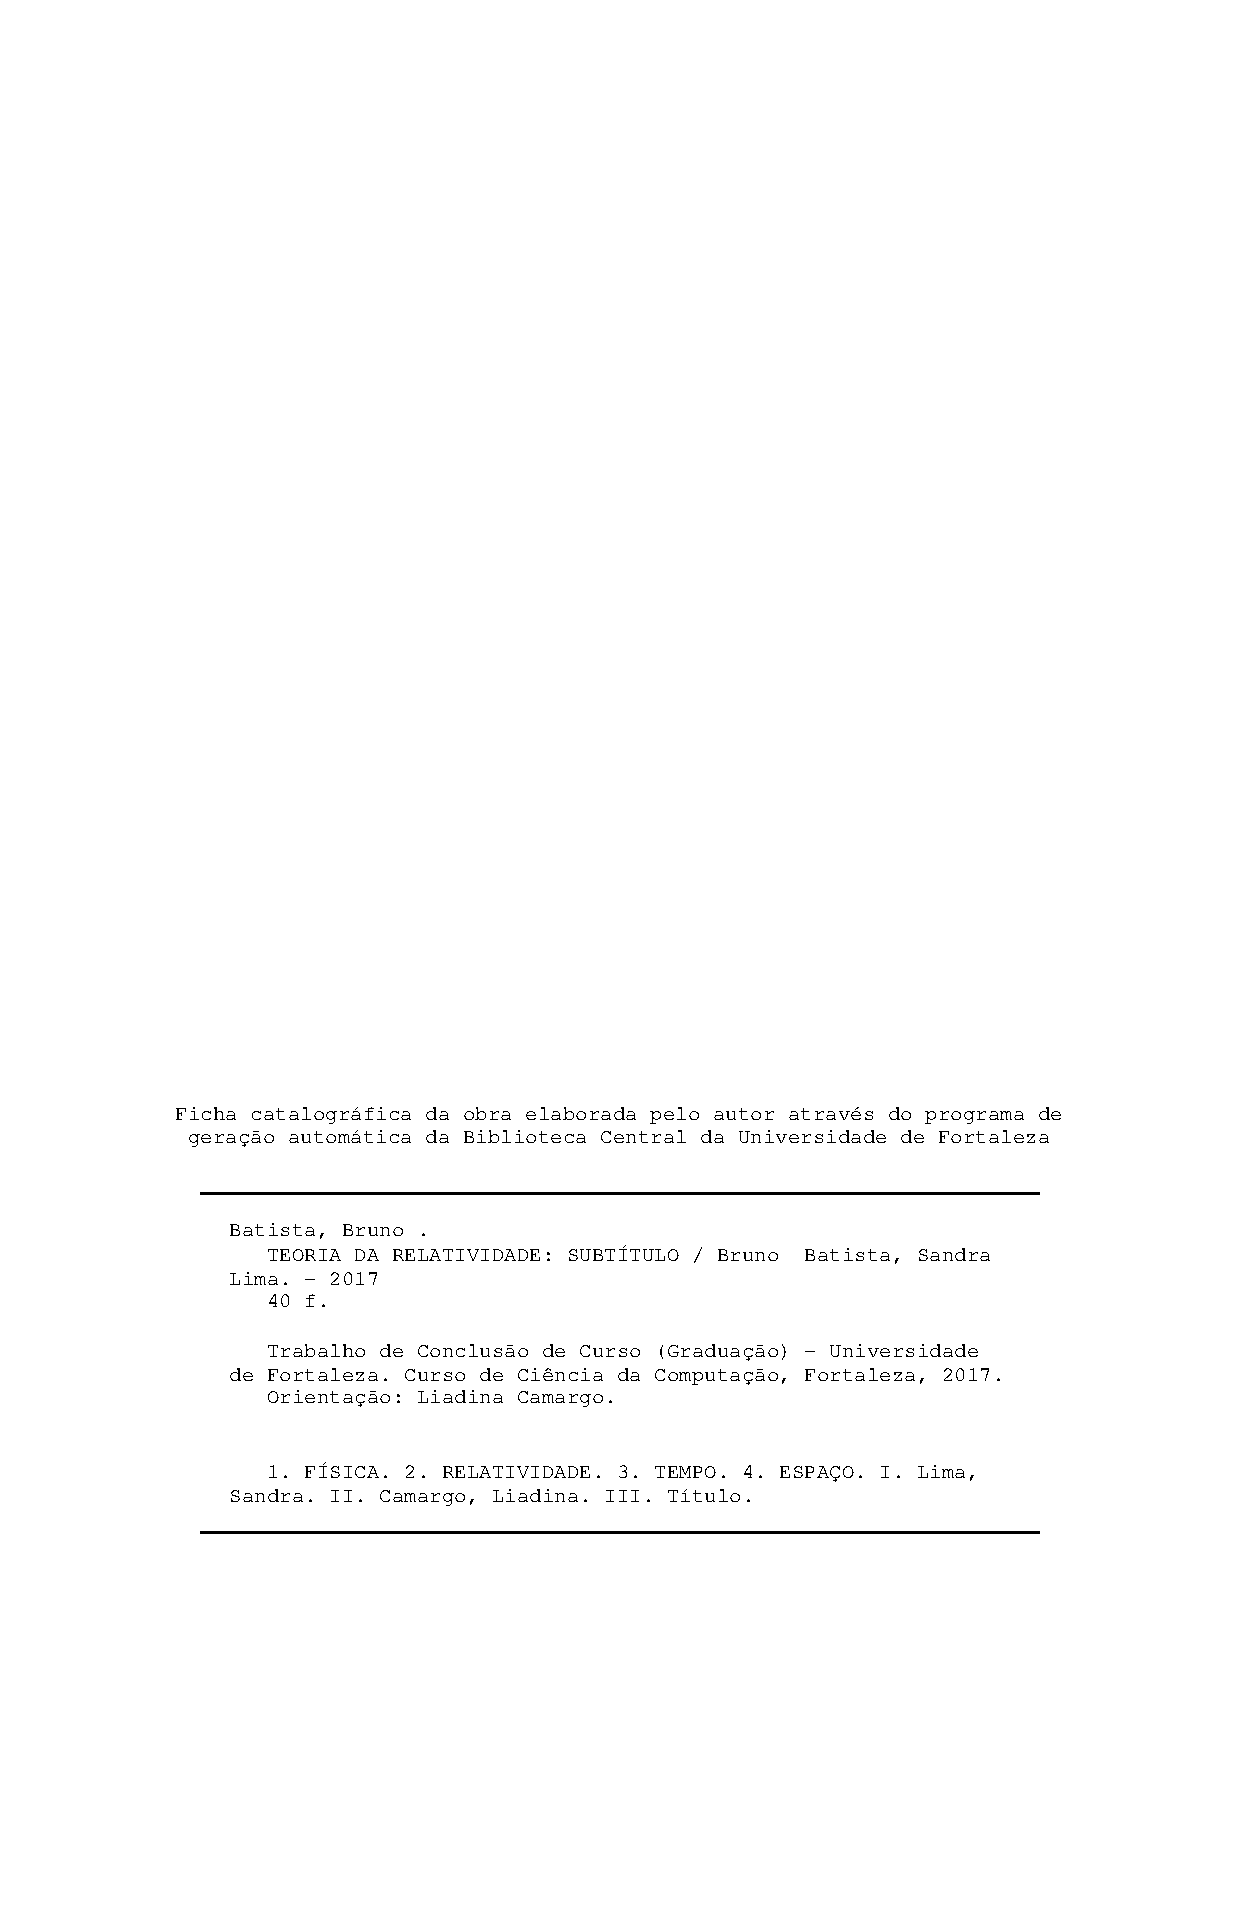
\includepdf{elementos-pre-textuais/folha-aprovacao.pdf}
		\imprimirfolhadeaprovacao

		\imprimirdedicatoria{elementos-pre-textuais/dedicatoria}
		\imprimiragradecimentos{elementos-pre-textuais/agradecimentos}
		\imprimirepigrafe{elementos-pre-textuais/epigrafe}
		\imprimirresumo{elementos-pre-textuais/resumo}
		\imprimirabstract{elementos-pre-textuais/abstract}
	\fi

	% Listas e sumário (comuns aos dois modos; cada lista sai vazia se o
	% documento não tiver o elemento correspondente).
	\imprimirlistadeilustracoes
	\imprimirlistadetabelas
	\imprimirlistadequadros
	\imprimirlistadealgoritmos
	\imprimirlistadecodigosfonte
	\imprimirlistadeabreviaturasesiglas
	\imprimirlistadesimbolos{elementos-pre-textuais/lista-de-simbolos}
	\imprimirsumario

	% Elementos textuais
	\textual
	\chapter{Introdução}
\label{cap:introducao}

% Descreva aqui o contexto geral do trabalho, apresentando o tema,
% a problemática e a justificativa da pesquisa.

% [Insira o texto da introdução aqui]

\section{Justificativa}
\label{sec:justificativa}

% Apresente a relevância e a motivação para a realização deste trabalho.

% [Insira a justificativa aqui]

\section{Objetivos}
\label{sec:objetivos}

% Apresente os objetivos geral e específicos do trabalho.

\subsection{Objetivo Geral}
\label{sec:objetivo-geral}

% [Insira o objetivo geral aqui]

\subsection{Objetivos Específicos}
\label{sec:objetivos-especificos}

% Liste os objetivos específicos usando alíneas:
%
% \begin{alineas}
% 	\item Objetivo específico 1;
% 	\item Objetivo específico 2;
% 	\item Objetivo específico 3.
% \end{alineas}

% [Insira os objetivos específicos aqui]
	\chapter{Revisão de Literatura}
\label{cap:revisao-de-literatura}

% Apresente aqui a fundamentação teórica do trabalho.
% Realize uma revisão bibliográfica dos principais conceitos,
% teorias e trabalhos anteriores relacionados ao tema.

% [Insira o texto da revisão de literatura aqui]

\section{Tema A}
\label{sec:tema-a}

% [Insira o conteúdo da primeira seção aqui]

% Dica: Para inserir uma figura, use o seguinte modelo:
%
% \begin{figure}[!htbp]
%     \centering
%     \EMBRAPAfig{
%         \Caption{\label{fig:exemplo} Legenda da figura}
%     }{
%         \includegraphics[width=8cm]{figuras/nome-da-figura}
%     }{
%         \Fonte{Elaborado pelo autor}
%     }
% \end{figure}

\section{Tema B}
\label{sec:tema-b}

% [Insira o conteúdo da segunda seção aqui]

% Dica: Para inserir uma tabela, use o seguinte modelo:
%
% \begin{table}[!htbp]
%     \centering
%     \Caption{\label{tab:exemplo} Legenda da tabela}
%     \EMBRAPAtab{}{
%         \begin{tabular}{cll}
%             \toprule
%             Coluna 1 & Coluna 2 & Coluna 3 \\
%             \midrule \midrule
%             Dado 1 & Dado 2 & Dado 3 \\
%             \bottomrule
%         \end{tabular}
%     }{
%         \Fonte{Elaborado pelo autor}
%     }
% \end{table}

	\chapter{Estado da Arte}
\label{cap:estado-da-arte}

% Apresente aqui uma revisão dos trabalhos e pesquisas mais recentes
% relacionados ao tema, destacando as contribuições e lacunas existentes.

% [Insira o texto do estado da arte aqui]

\section{Trabalho/Pesquisa A}
\label{sec:trabalho-a}

% [Descreva o primeiro trabalho relacionado]

\section{Trabalho/Pesquisa B}
\label{sec:trabalho-b}

% [Descreva o segundo trabalho relacionado]

% Dica: Para inserir um quadro comparativo, use o seguinte modelo:
%
% \begin{quadro}[!htbp]
%     \centering
%     \Caption{\label{qua:comparativo} Legenda do quadro}
%     \EMBRAPAqua{}{
%         \begin{tabular}{|c|c|c|}
%             \hline
%             Critério & Trabalho A & Trabalho B \\
%             \hline
%             Critério 1 & Valor & Valor \\
%             \hline
%         \end{tabular}
%     }{
%         \Fonte{Elaborado pelo autor}
%     }
% \end{quadro}

	\chapter{Material e Métodos}
\label{cap:material-e-metodos}

% Descreva aqui os materiais utilizados e os métodos empregados
% na realização da pesquisa. Inclua informações sobre:
% - Área de estudo / local do experimento
% - Materiais e equipamentos
% - Delineamento experimental
% - Procedimentos analíticos
% - Análises estatísticas

% [Insira o texto de material e métodos aqui]

\section{Área de Estudo}
\label{sec:area-de-estudo}

% [Descreva a área ou local onde o trabalho foi realizado]

\section{Procedimentos Metodológicos}
\label{sec:procedimentos-metodologicos}

% [Descreva os procedimentos utilizados]

% Dica: Para inserir um algoritmo, use o seguinte modelo:
%
% \begin{algorithm}[h!]
%     \SetSpacedAlgorithm
%     \caption{\label{alg:exemplo}Descrição do Algoritmo}
%     \Entrada{Entrada do Algoritmo}
%     \Saida{Saída do Algoritmo}
%     \Inicio{
%         Passo 1\;
%         Passo 2\;
%     }
% \end{algorithm}

\section{Análise dos Dados}
\label{sec:analise-dos-dados}

% [Descreva como os dados foram analisados]

% Dica: Para inserir fórmulas matemáticas:
%
% \begin{equation}
%     \begin{aligned}
%         y = ax + b
%     \end{aligned}
% \end{equation}

	\chapter{Resultados e Discussão}
\label{cap:resultados-e-discussao}

% Apresente aqui os resultados obtidos na pesquisa e discuta-os
% à luz da literatura revisada. Inclua figuras, tabelas e gráficos
% conforme necessário.

% [Insira os resultados e a discussão aqui]

\section{Resultados}
\label{sec:resultados}

% [Apresente os resultados obtidos]

\section{Discussão}
\label{sec:discussao}

% [Discuta os resultados à luz da literatura]

	\chapter{Considerações Finais}
\label{cap:consideracoes-finais}

% Apresente aqui as conclusões do trabalho, retomando os objetivos
% propostos e avaliando se foram alcançados.

% [Insira as considerações finais aqui]

\section{Contribuições do Trabalho}
\label{sec:contribuicoes-do-trabalho}

% [Descreva as principais contribuições]

\section{Limitações}
\label{sec:limitacoes}

% [Descreva as limitações encontradas]

\section{Recomendações e Trabalhos Futuros}
\label{sec:recomendacoes-e-trabalhos-futuros}

% [Apresente recomendações e sugestões para trabalhos futuros]


	% Elementos pós-textuais
	% Todos abaixo aparecem no PDF SOMENTE quando há conteúdo correspondente;
	% caso contrário, são omitidos automaticamente (sem título em página vazia).

	% Referências: impressas se houver \cite/\citeonline no texto. Para forçar
	% a inclusão de uma obra não citada (ex.: a norma ABNT NBR 14724), adicione
	% \nocite{NBR14724:2005} antes da linha abaixo.
	\imprimirreferencias{elementos-pos-textuais/referencias}

	% Glossário: impresso se algum termo do glossário principal for usado no
	% texto com \gls/\Gls (siglas vão para a Lista de Abreviaturas e Siglas).
	\imprimirglossario

	% Apêndices: passe os \input dentro das chaves. Deixe vazio para omitir.
	\imprimirapendices{%
		\apendice{Exemplo de Apêndice}
\label{ap:exemplo-de-apendice}

% Apêndice é um texto ou documento elaborado pelo autor.
% Adicione aqui o conteúdo do apêndice.

% [Insira o conteúdo do apêndice aqui]
Este apêndice apresenta material complementar elaborado pelo autor, como dados adicionais, formulários ou detalhamentos que apoiam o texto principal sem comprometer a sua fluidez.
%
	}

	% Anexos: passe os \input dentro das chaves. Deixe vazio para omitir.
	\imprimiranexos{%
		\anexo{Exemplo de Anexo}
\label{an:exemplo-de-anexo}

% Anexo é um texto ou documento não elaborado pelo autor.
% Adicione aqui o conteúdo do anexo.

% [Insira o conteúdo do anexo aqui]%
	}

	% Índice remissivo: impresso apenas se houver entradas \index{} no texto.
	\imprimirindice

\end{document}
